\documentclass[12pt,righttag]{article}

\usepackage{amssymb}
\usepackage{graphicx}

\begin{document}
	\title{Two Electrons in a Harmonic Oscillator Potential}
	\author{Sean Sweany}
	\renewcommand{\today}{April 3, 2016}
	\maketitle
	
	\begin{abstract}
Many body problems are used in describing everything from things on the smallest scale (quantum mechanics, molecular dynamics) to those the largest scale (solar system, galactic dynamics). A model of our solar system was made using two separate methods for solving the differential equations governing Newtonian gravity, a fourth order Runge Kutta, and the Verlet method. The code for each was slowly built up starting by hard coding then generalizing this by using classes. To determine if the classes work correctly we slowly added planets to the system starting with the sun and earth then adding Jupiter and finally the entire solar system. The stability of these two methods was studied over extended periods of time in order to determine optimal step sizes and to compare the two methods. What was discovered however is that to truly have stability for an infinite amount of time the step size has to be so small that it becomes infeasible to run the code for any meaningful time period (by meaningful time period I guess that my definition of this is that for the whole solar system all of the planets need to be able to make several orbits around the sun).
	\end{abstract}

	
	\section{Introduction}
    Our solar system, as was learned in early grade school has nine planets (until they got rid of Pluto). So, for something which is so ingrained in all of us it just makes sense that we would want to understand how this system of nine orbiting planets works. An answer to this question was given by Isaac Newton in 1687 when he published the Principia which along with little things like calculus he also included his laws of motion [1]. These laws are what we use here to describe the motion of the planets as they orbit the sun. This classic many body problem is easily solved today by the help of computers. In this study we have only included the orbits in the x and y plane since for most of the planets except Pluto and Mercury their orbits are mostly circular in the x/y plane.


	
	\section{Theory}
Excluding things such as general relativity the motion of the planets can be described by the following differential equation:
\[F=\frac{-GM_1 M_2}{r^2}\]
 Where the two M's are for the masses of the two objects exerting the gravitational force, the r is just the separation between the two bodies and G is the gravitational constant. So for the system containing only the sun and the earth where the sun doesn't move we have the following two differential equations to solve.
 \[\frac{d^2x}{dt^2}=\frac{F_x}{M_{earth}}\]
 
 and
  \[\frac{d^2y}{dt^2}=\frac{F_y}{M_{earth}}\]
  Right now these two equations for the acceleration in the x and y directions are both second order differential equations, however these can be broken down into four first order equations. Take the differential equation for x, set $\frac{d^2x}{dt^2}=\frac{dv_x}{dt}$ and $\frac{dv_x}{dt}=x$. Doing the same thing to y gives four first order differential equations (just as a note for $F_x$ all this is is just F except now multiplied by cos, which is just x/r, same for $F_y$ except now we use sine) Now, the next thing is that the function for the force above has both the mass of the planets and G in it, where the masses are very large and G is very small. These large and small numbers can make it difficult for the program to actually run. So since we are assuming circular orbits, we can use the simple equation for acceleration which was learned in our basic physics classes $\frac{v^2}{r}$. This gives us that
  \[F=\frac{-M_{earth}v^2}{r}=\frac{-GM_{earth}M_{sun}}{r^2}\]
  So $GM_{sun}=v^2r$, and using that the distance scale being used is just AU's and that the time is simply years we have that r=1 and $v^2=4\pi^2$. This give us that $GM_{sun}=4\pi^2$. So, in the end the four differential equations that need to be solved are simply just
  \[\frac{dx}{dt}=v_x,    \frac{dy}{dt}=v_y\]
  \[\frac{dv_x}{dt}=\frac{-4\pi^2(x_{earth}-x_{sun})}{r^3}, \frac{dv_y}{dt}=\frac{-4\pi^2(y_{earth}-y_{sun})}{r^3}\]
  
  For extending these equations is simple, all that needs to be done is all other planets interacting with the sun have the same equation, and for the planets interacting with them selves simply have multiplied the ratio of the acting planet to that of the sun. This simple is just showing how much influence the planets gravity has over the other planet as compared the that of the sun.[1][2][3]
 
\section{Numerical Methods}
In this project two different differential equation solvers were used to solve the solar system problem. These are the Verlet Method and the fourth order Runge Kutta method. I am not going to go very in depth in the derivation of these to methods since they are both fairly common (especially Runge Kutta). So starting off with the Verlet Method, or in our case we are using what's called the Velocity Verlet Algorithm. The derivation of this is very similar to that of the different Euler methods, where you take Taylor series and do clever manipulations with them until you arrive at a solution which for the Velocity Verlet is 
\[x_{i+1}=x_i+hv_i+\frac{h^2}{2}F_i+O(h^3)\]
and
\[v_{i+1}=v_i+\frac{h}{2}(F_{i+1}+F_i)+O(h^3)\]

Looking at the equations we can see that they have the significant advantage over the Euler methods discussed so far as in they are of third order equations.


The next method is the fourth order Runge Kutta method. Now, the Runge Kutta methods are interesting in the fact that they are completely different from any of the ways we have discussed in solving differential equation previously. The previous differential equation solvers we have talked about come from simple tricks with Taylor series and are all rather cute. The Runge Kutta methods do come from Taylor series but are based on making a prediction of the value at the next step and then making corrections to this prediction. The higher the order of the Runge Kutta method the more corrections made and the better the accuracy, this of course comes at the expense of more computing time. The fourth Runge Kutta method being used is 
\[k_1=F(t_i,x_i)\]
\[k_2=F(t_i+h/2,x_i+k_1/2)\]
\[k_3=F(t_i+h/2, x_i+k_2/2)\]
\[k_4=F(t_i+h, x_i+k_3)\]
\[x_{i+1}=x_i+(1/6)(k_1+2k_2+2k_3+k_4)\]
this is of course for only one differential equation. For our present case we have four coupled differential equations for the F's will be functions of $x, y,v_x,v_y$, and each will have it's own k's.[2]





\section{Results}
\subsection{The Earth Sun Interaction}
The first system studied with the two methods was the Earth/Sun system, where the Sun is held in a constant position. For this system refer to Fig. ~\ref{OrbitEarth}, which is the motion of the earth around the Sun for 100 years. For this plot the initial conditions for the earth were chosen to be at a distance of 1Au in the x direction and a velocity of $2\pi$ in the y direction, it was found that these values give a circular orbit. A step size of 0.001 was used.
\begin{figure}
	\begin{center}
		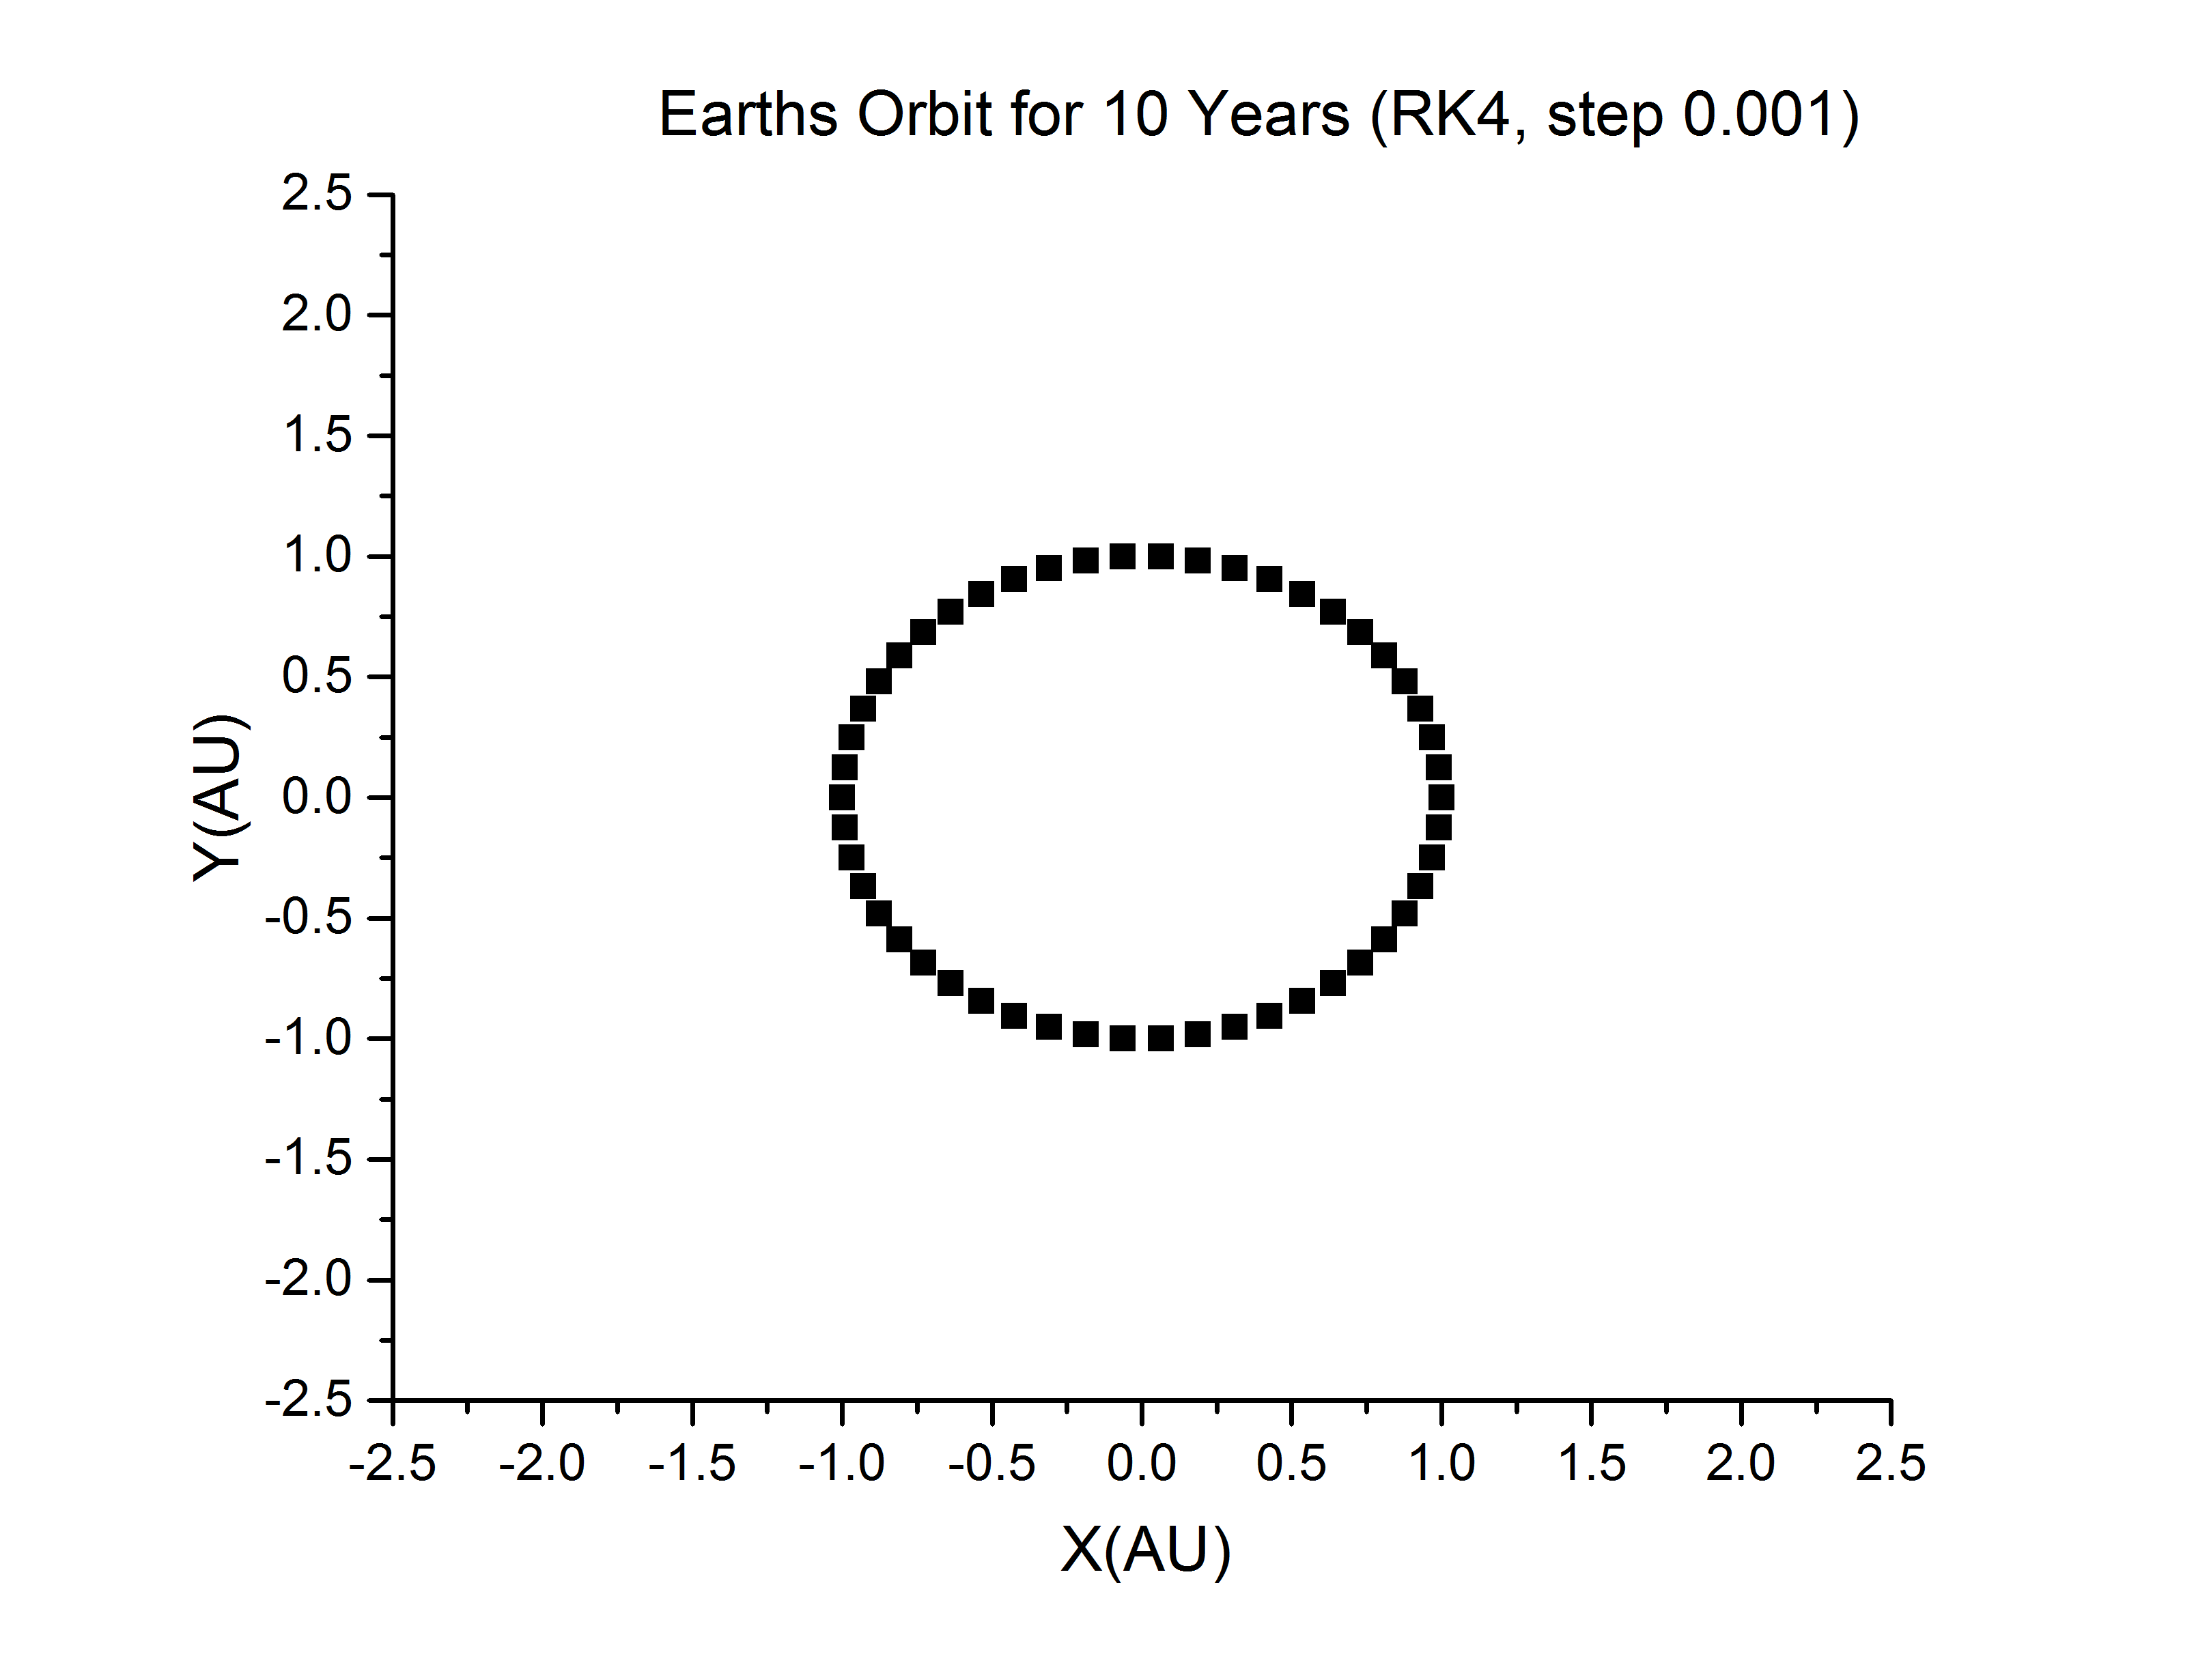
\includegraphics[width=3in]{Graph1.png}
		\caption{\label{OrbitEarth} Orbit or the earth around the sun. }
		\end{center}
	\end{figure}	
 Now, it was found that this step size isn't totally stable for the Runge Kutta or Verlet algorithms as can be seen in Fig. ~\ref{Stability}. Looking at this figure it is apparent that for both methods at a step size of 0.001 the difference in the initial and final energy is slowly increasing over the course of 100 years. Even trying a step size of 0.0001 showed that the energy differnce was increasing, however now it was in a very erratic and nonlinear way. The same results were found for the momentum as well. So even though the momentum and energy are not conserved for the step size of 0.001 I believe that this step size is appropriate to use because the amount that the energy is increasing in both methods is very small over the course of 100 years. However, this in not the ideal situation since by conservation laws both should be constant but making the step size any smaller makes it impossible for the code to run on my laptop for any length of time. So I believe that this is the best compromise.


The next part is to determine at what velocity a planet at 1AU would need to escape it's orbit. Trial and error showed that once a velocity of over $2\pi$ was chosen the orbit started to become unstable. However, over the time scale I was looking at it never actually escaped. So to prove that at a velocity of over $2\pi$ the earth will eventually escape we can use a simple conservation of energy argument. As was discussed in the book by Marion and Thorton [4] on classical mechanics if a orbital system has a total energy of less than zero the orbit will be stable. However, if it is over this value the planet will fly away. So, taking the energy of the system and setting it to zero gives the boundary of when the earth will fly away. The equation is 
\[\frac{1}{2}M_{earth}v^2 - \frac{-4\pi^2M_{earth}}{r}+\frac{l^2}{2M_{earth}r^2}=0\]
Where there is a part from kinetic and potential energies, there is also a third part called the effective potential which comes from the angular momentum of the system. Solving for v gives us that $v=\frac{2\pi}{\sqrt{r}}$. So, what this means is that for the earth, if the velocity is over $2\pi$ then it will go flying away from the sun. It will just do so very slowly.




		
		\begin{figure}
				
	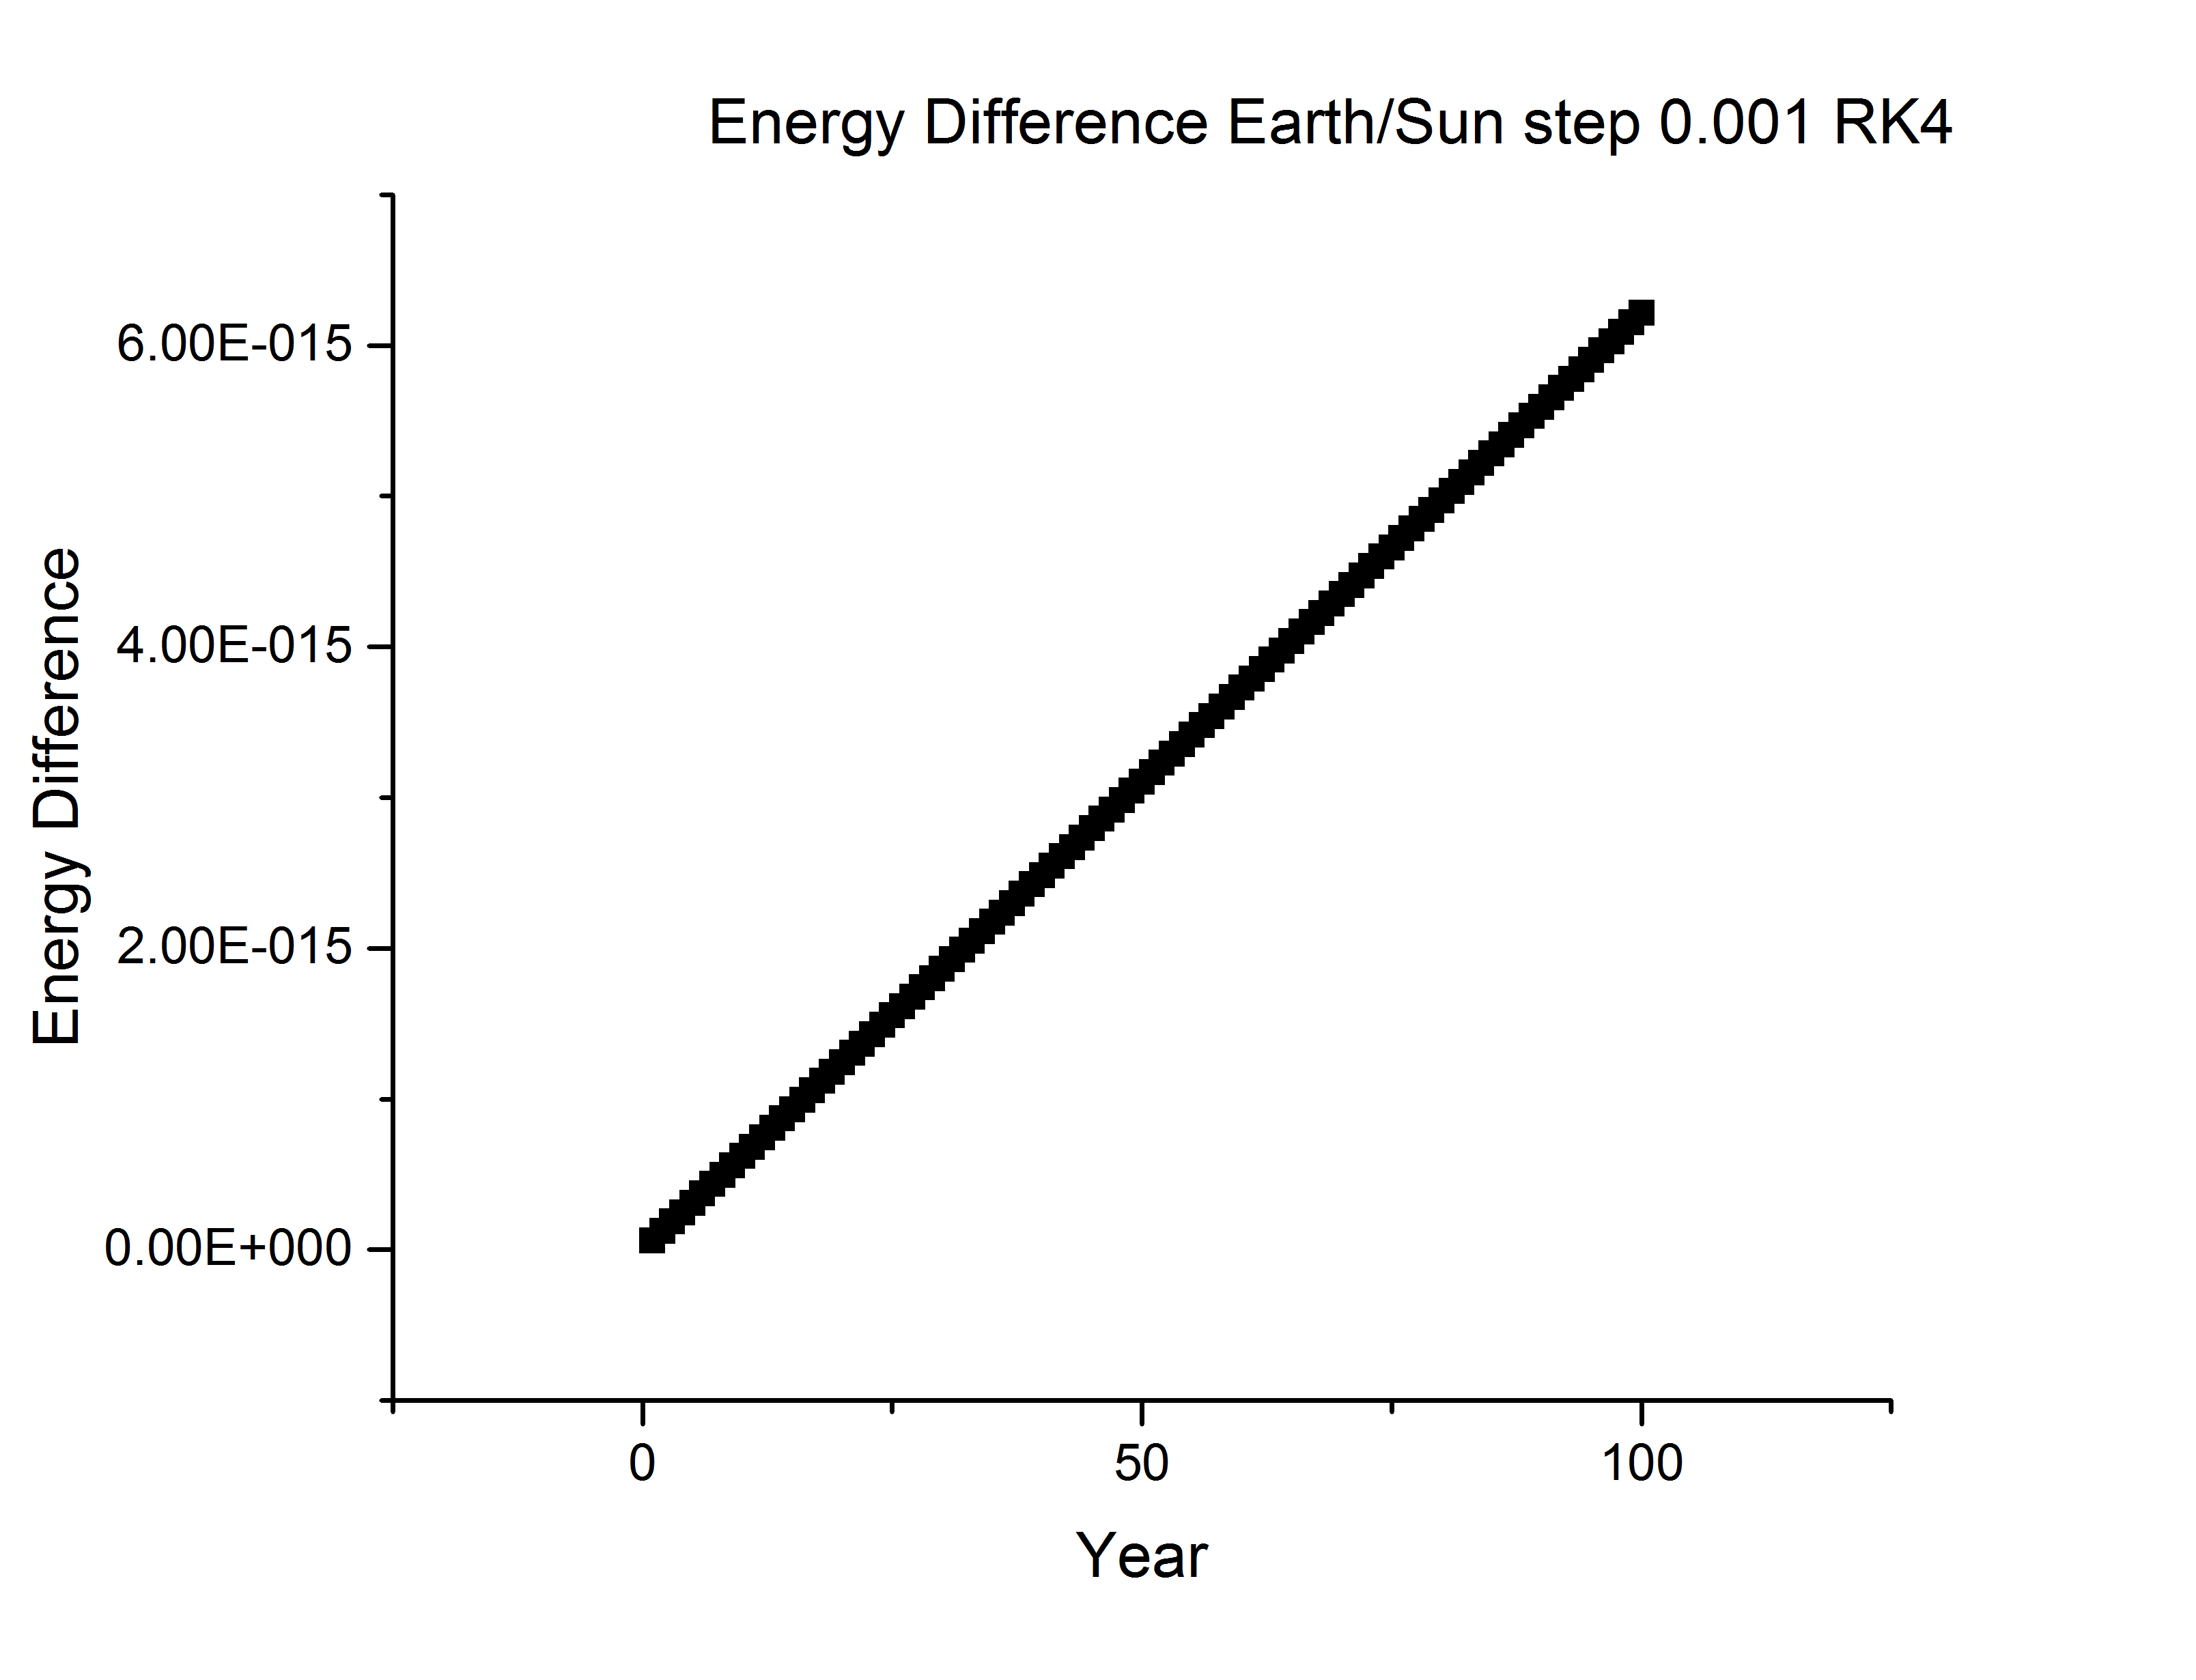
\includegraphics[width=3in]{Graph3.png}
	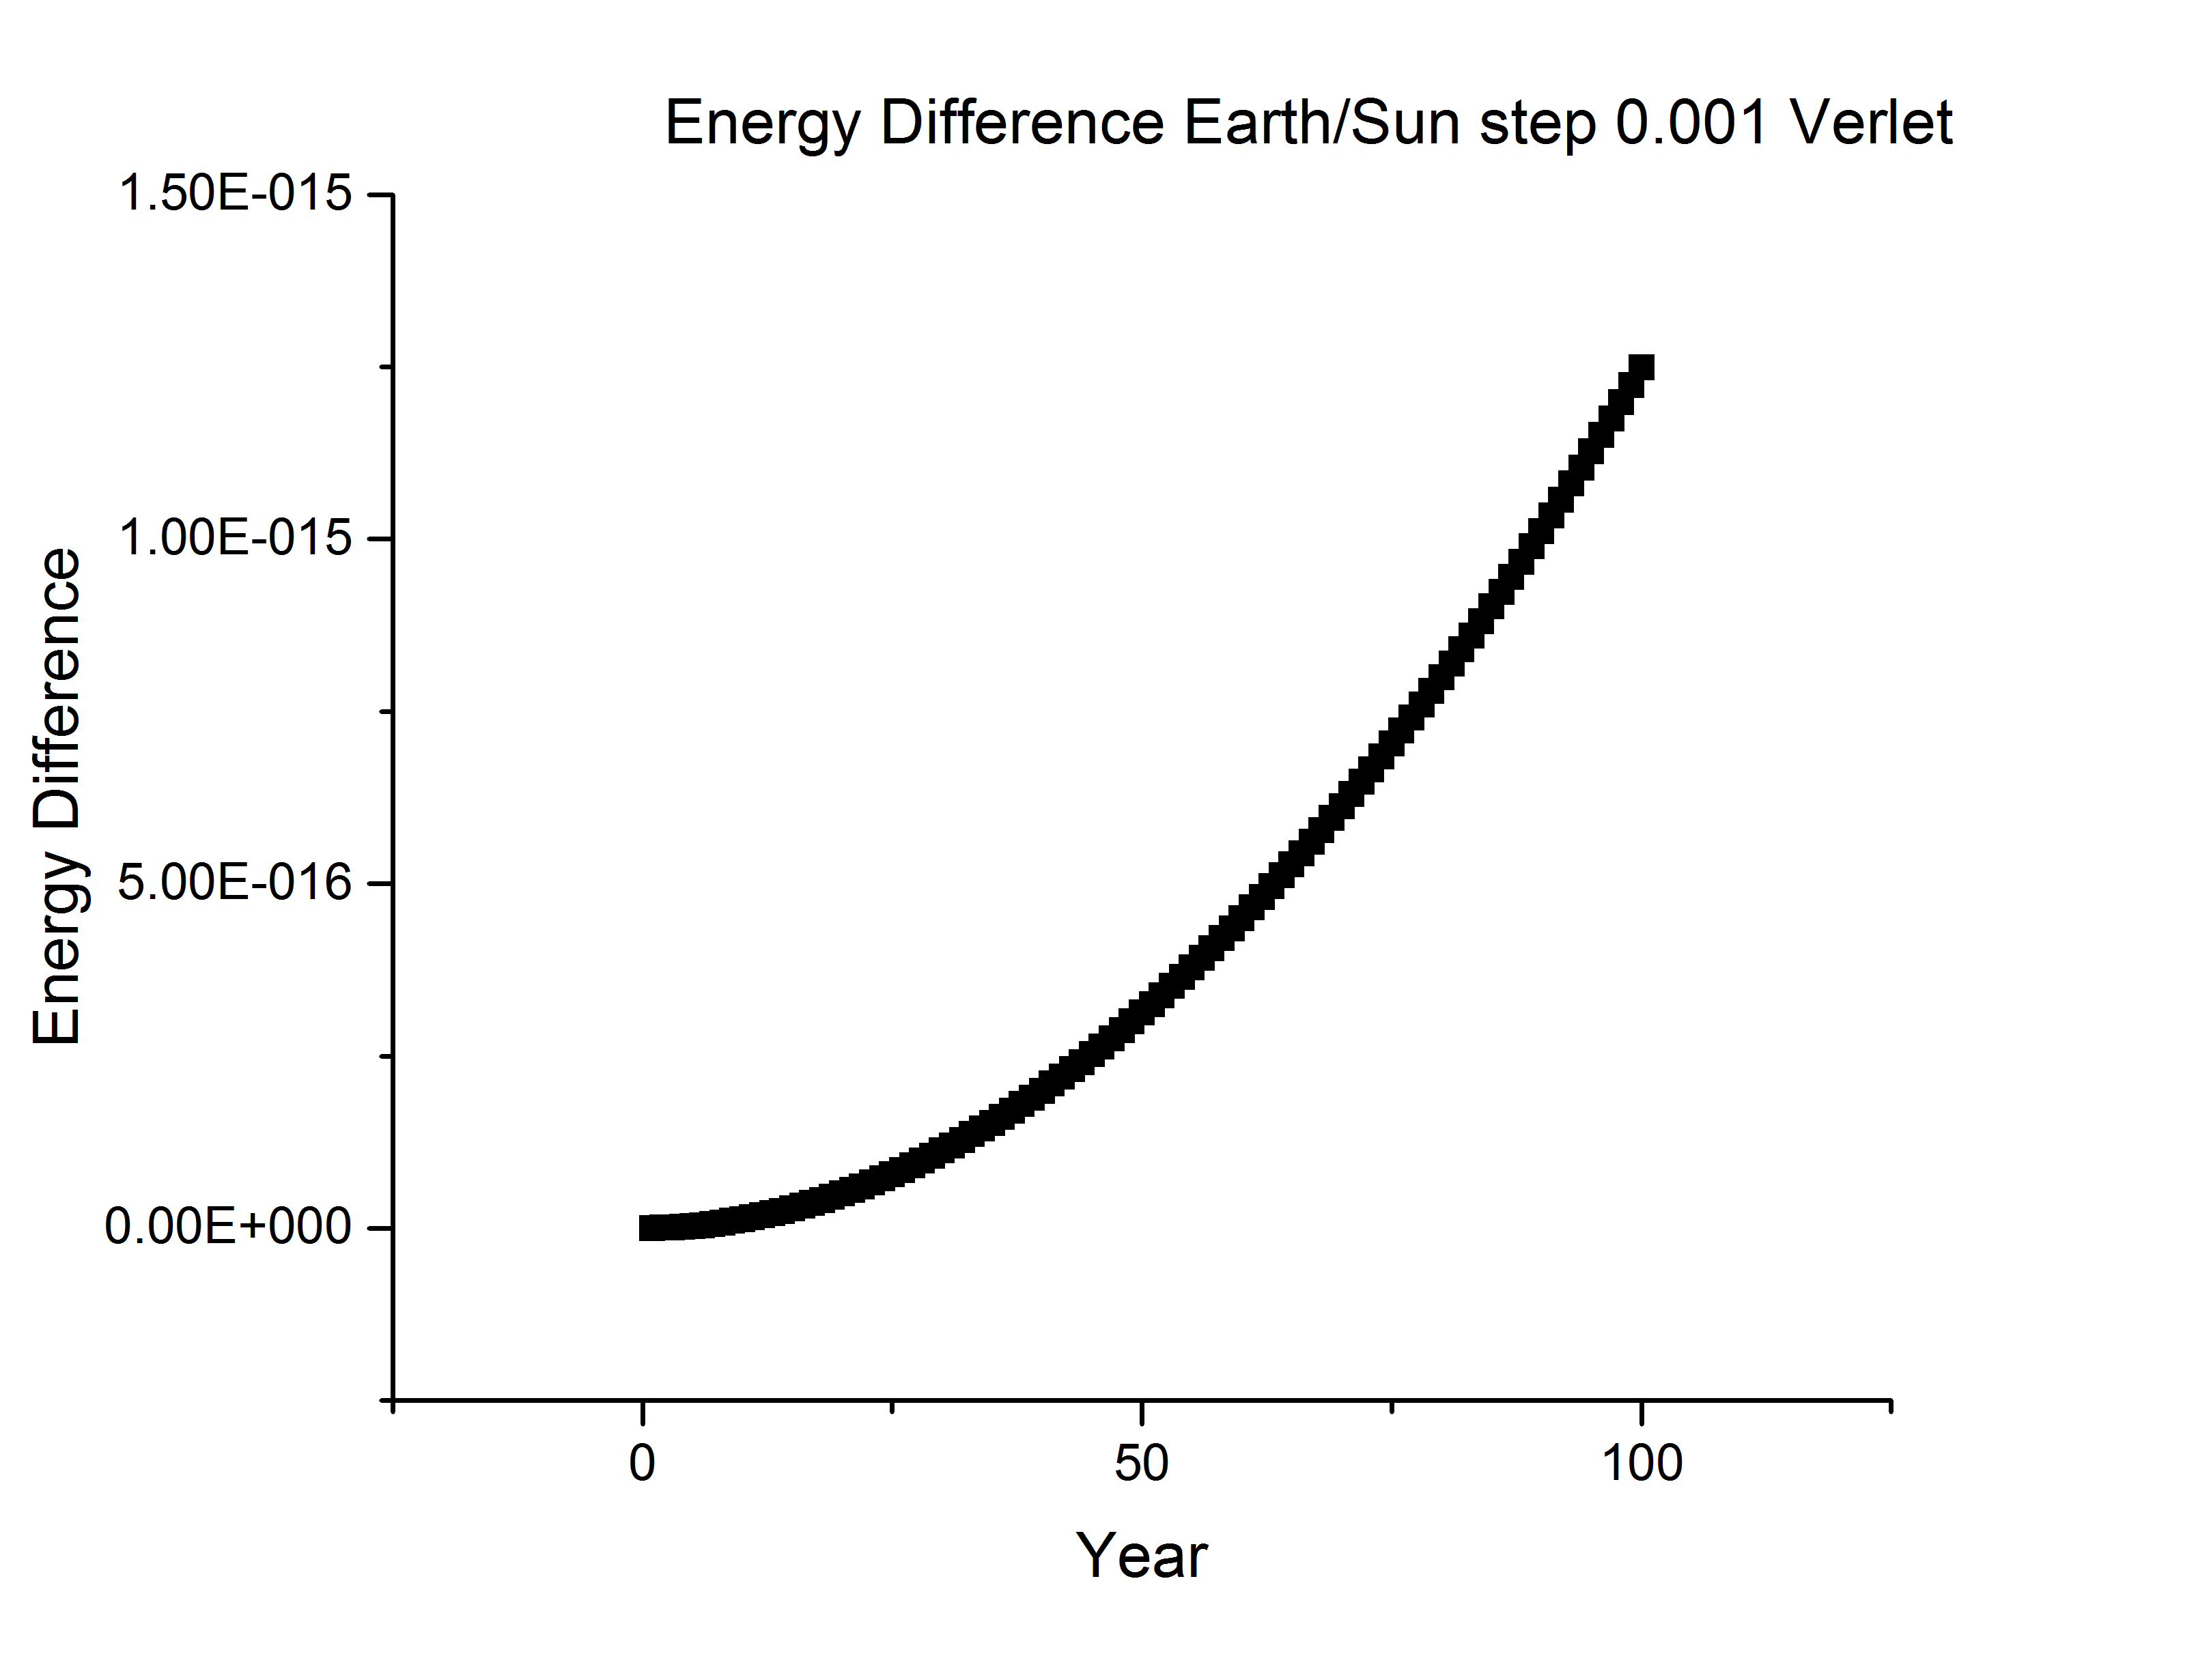
\includegraphics[width=3in]{Graph7.png}
		\caption{\label{Stability} Energy and Momentum difference for a step size of 0.001. }
		
		\end{figure}	
\subsection{Earth, Sun and Jupiter}
The next step is to now add Jupiter into the problem making a it a 3 body problem. To do this I used the initial velocity for Jupiter from by above equation, which actually is very close to what is obtained on the NASA website if only looking at the x and y direction. The interesting thing that was found is that when adding in Jupiter it actually makes the step size of 0.001 stable for both methods in terms of the energy difference refer to Fig.~\ref{Stability2}. From this figure it is clear that the energy difference is larger than in the sun and earth system however it is semi stable, bouncing between two values. The difference in the total momentum difference in increasing in both cases Fig.~\ref{Stability3}. In the Runge Kutta it is increasing linearly and for the Verlet it is increasing in a more sporadic manner, but is does look as though it may be leveling out.
\begin{figure}

	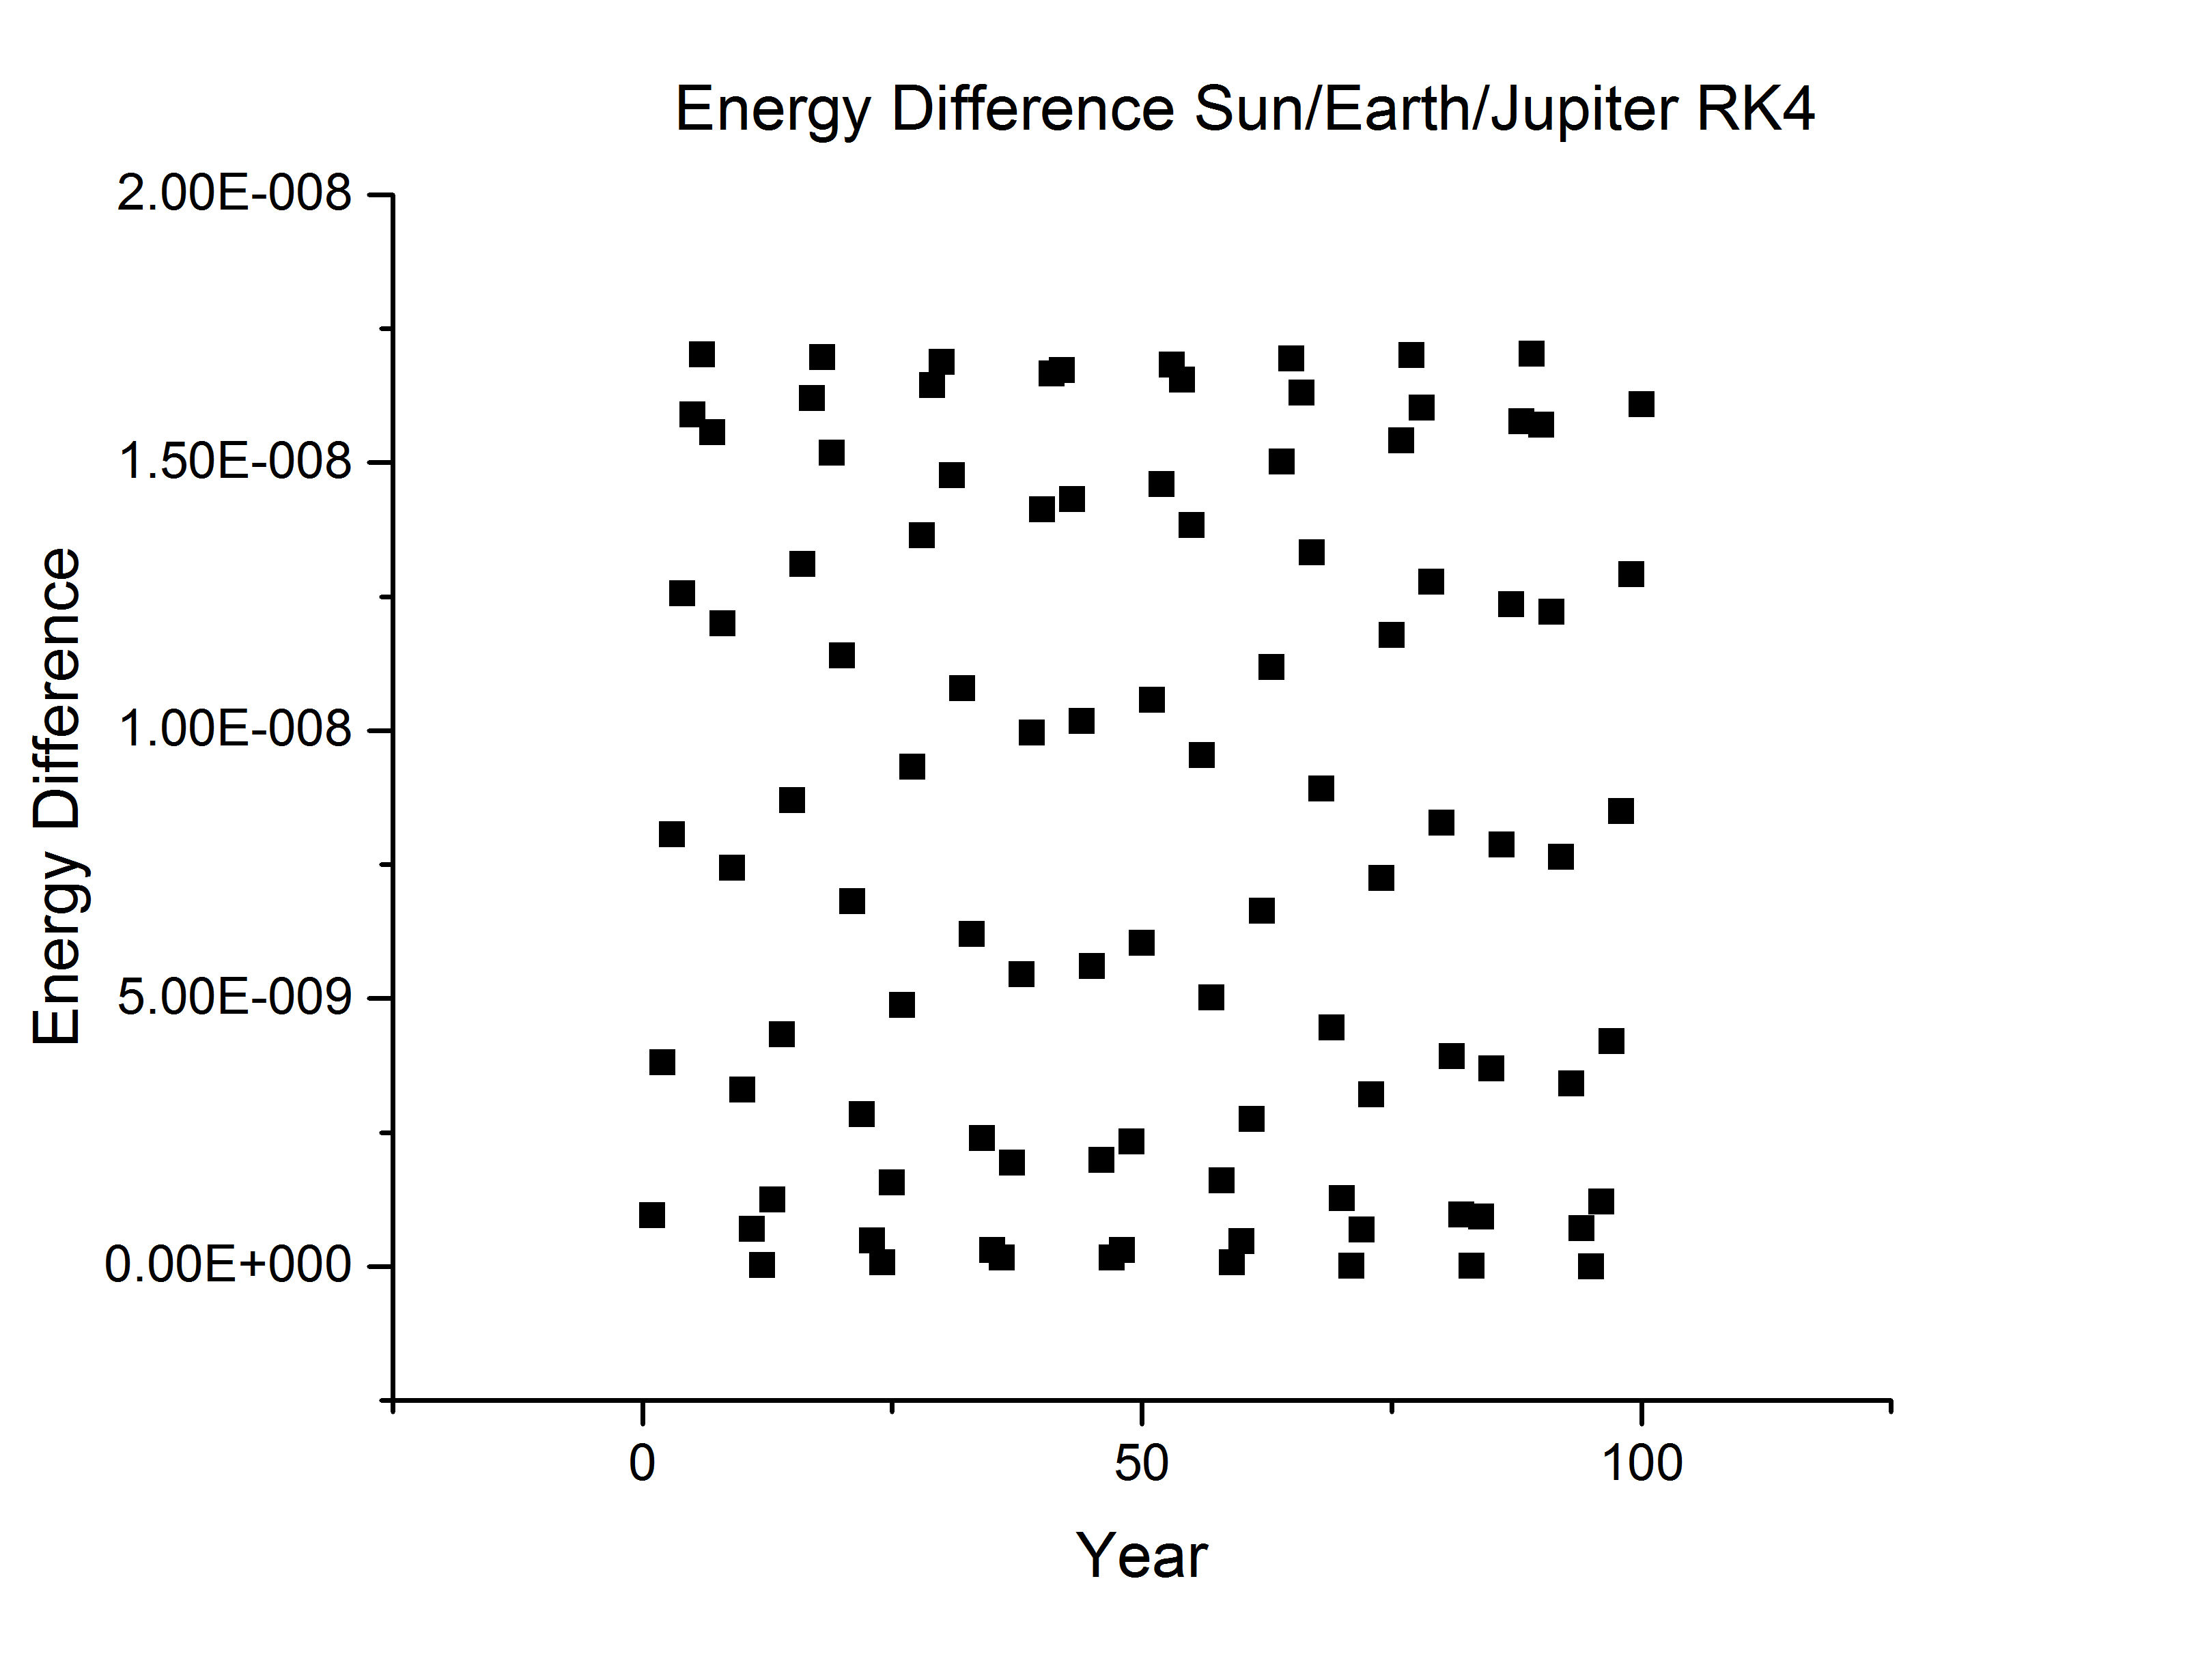
\includegraphics[scale=0.24]{Graph10.png}
	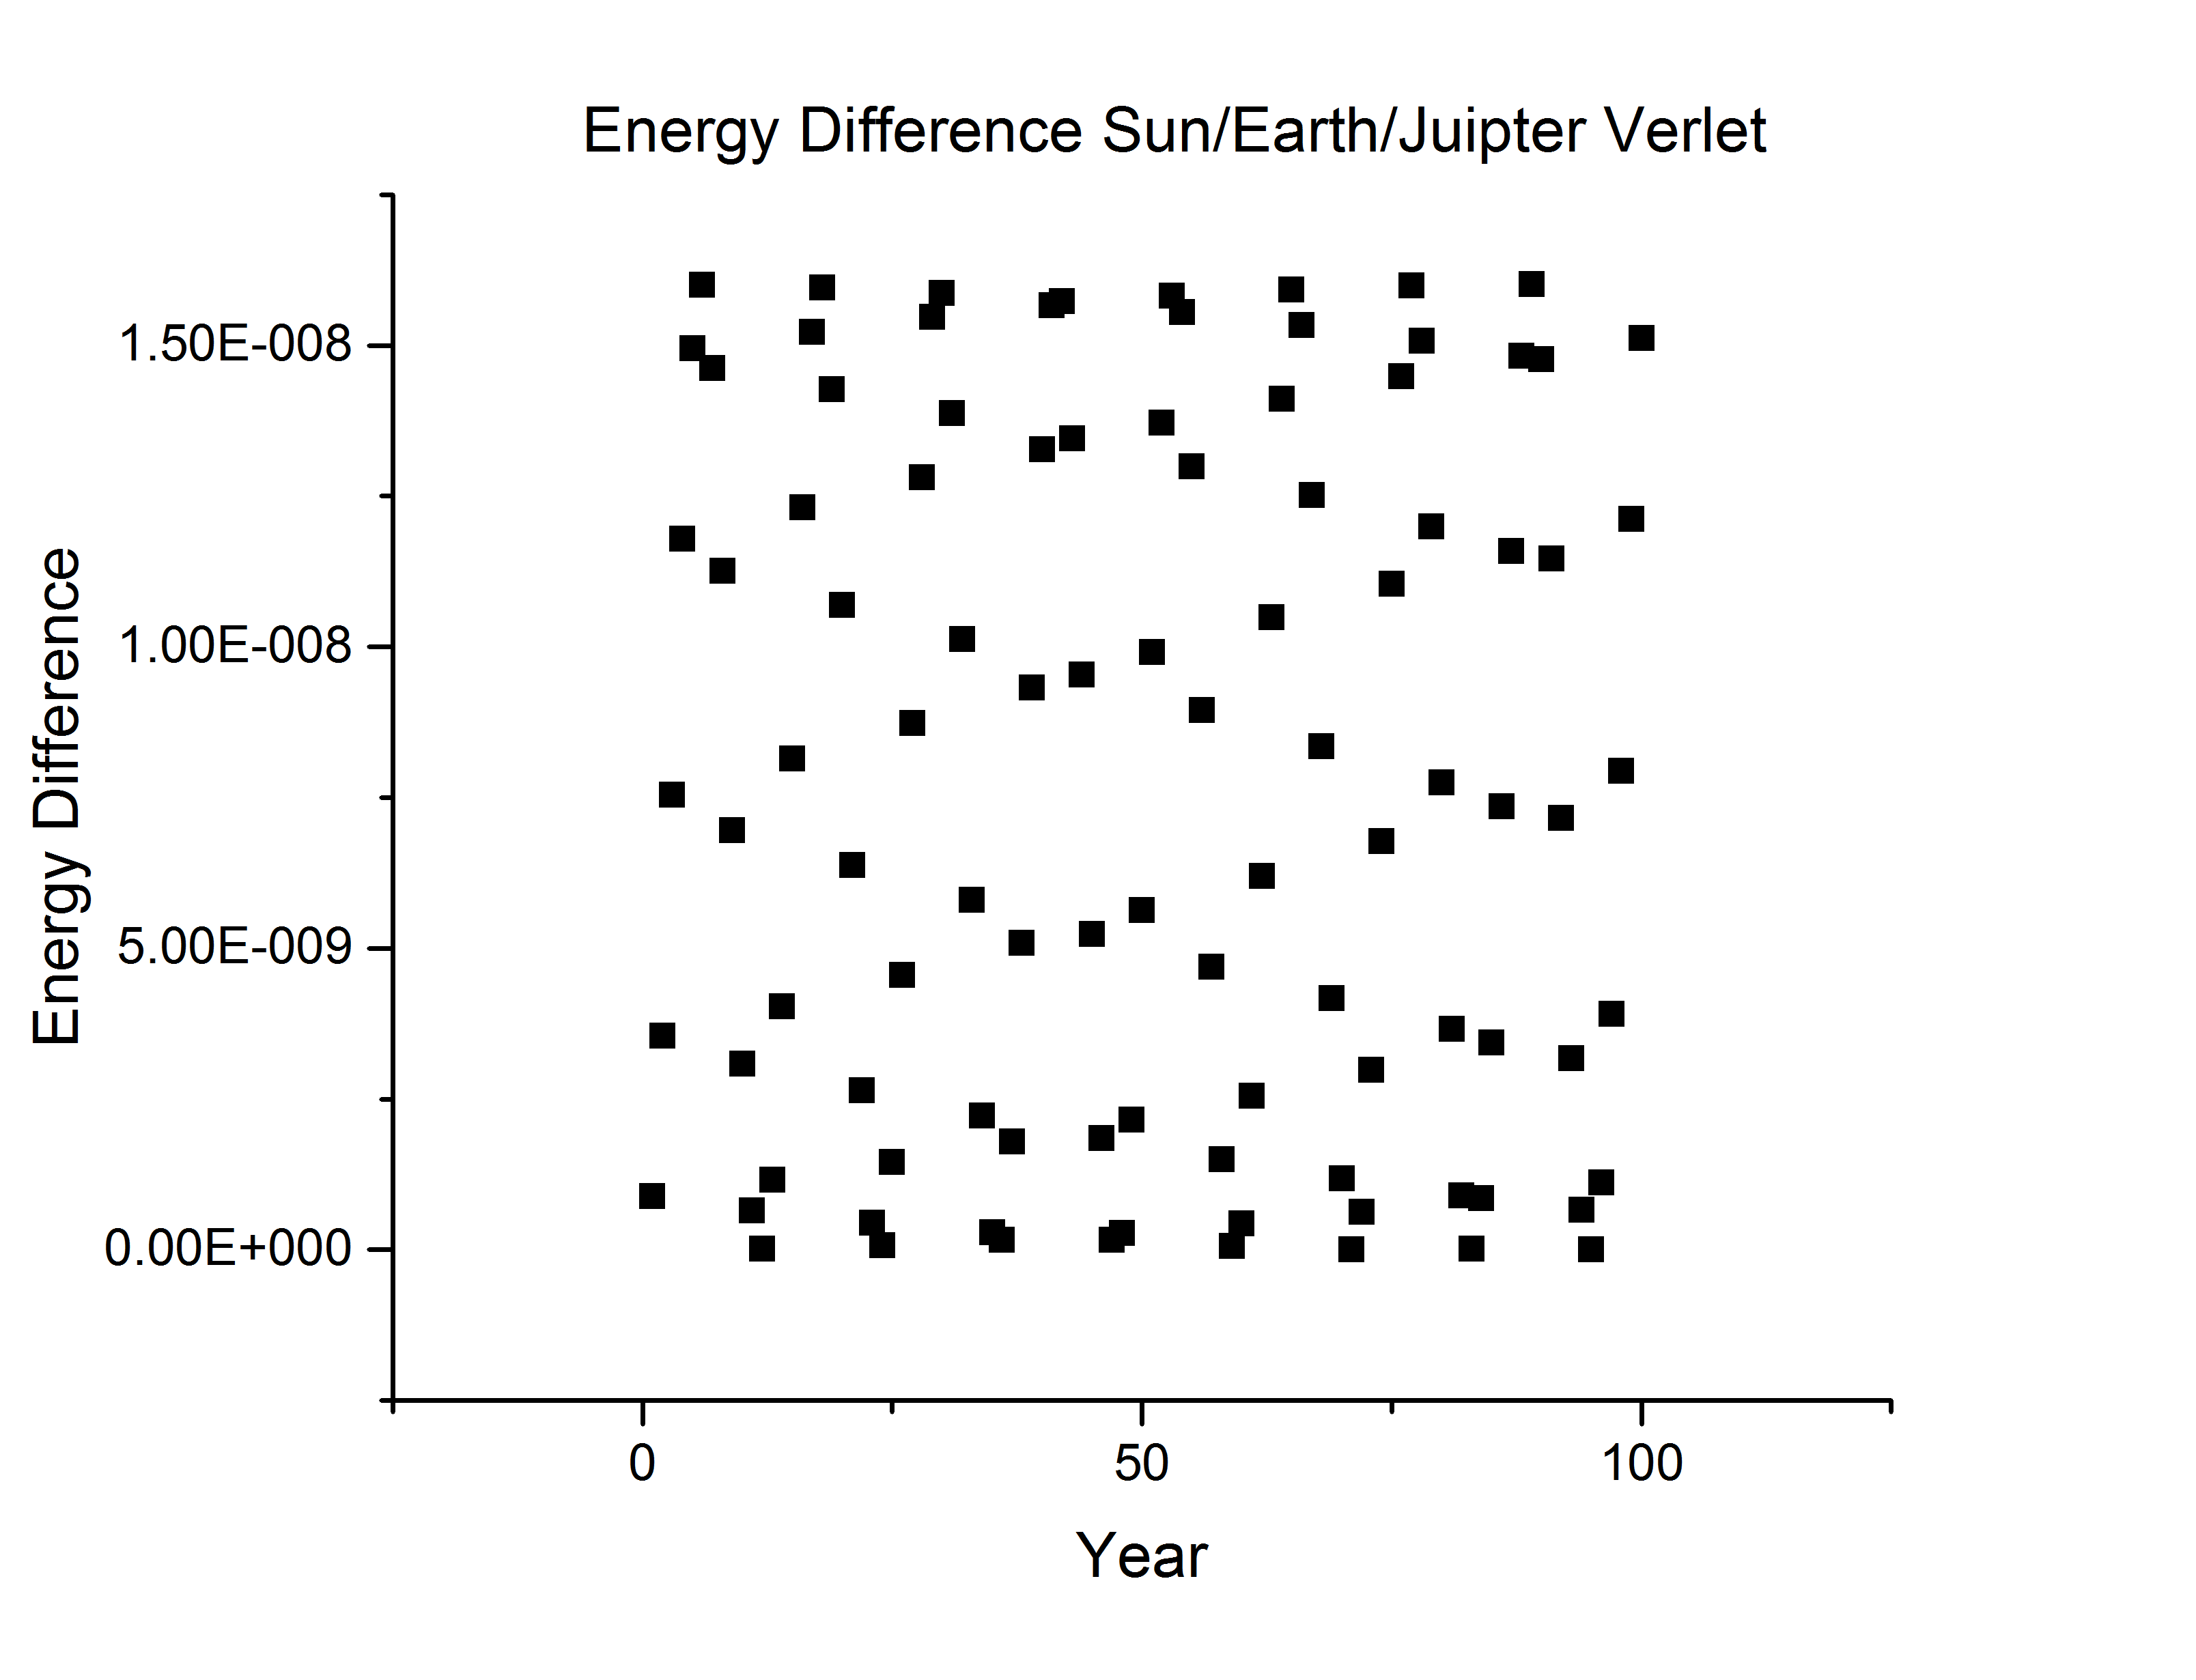
\includegraphics[scale=0.24]{Graph11.png}
	\caption{\label{Stability2} Energy difference for Sun/Earth/Jupiter step size 0.001. }
		\end{figure}		
		
			\begin{figure}
	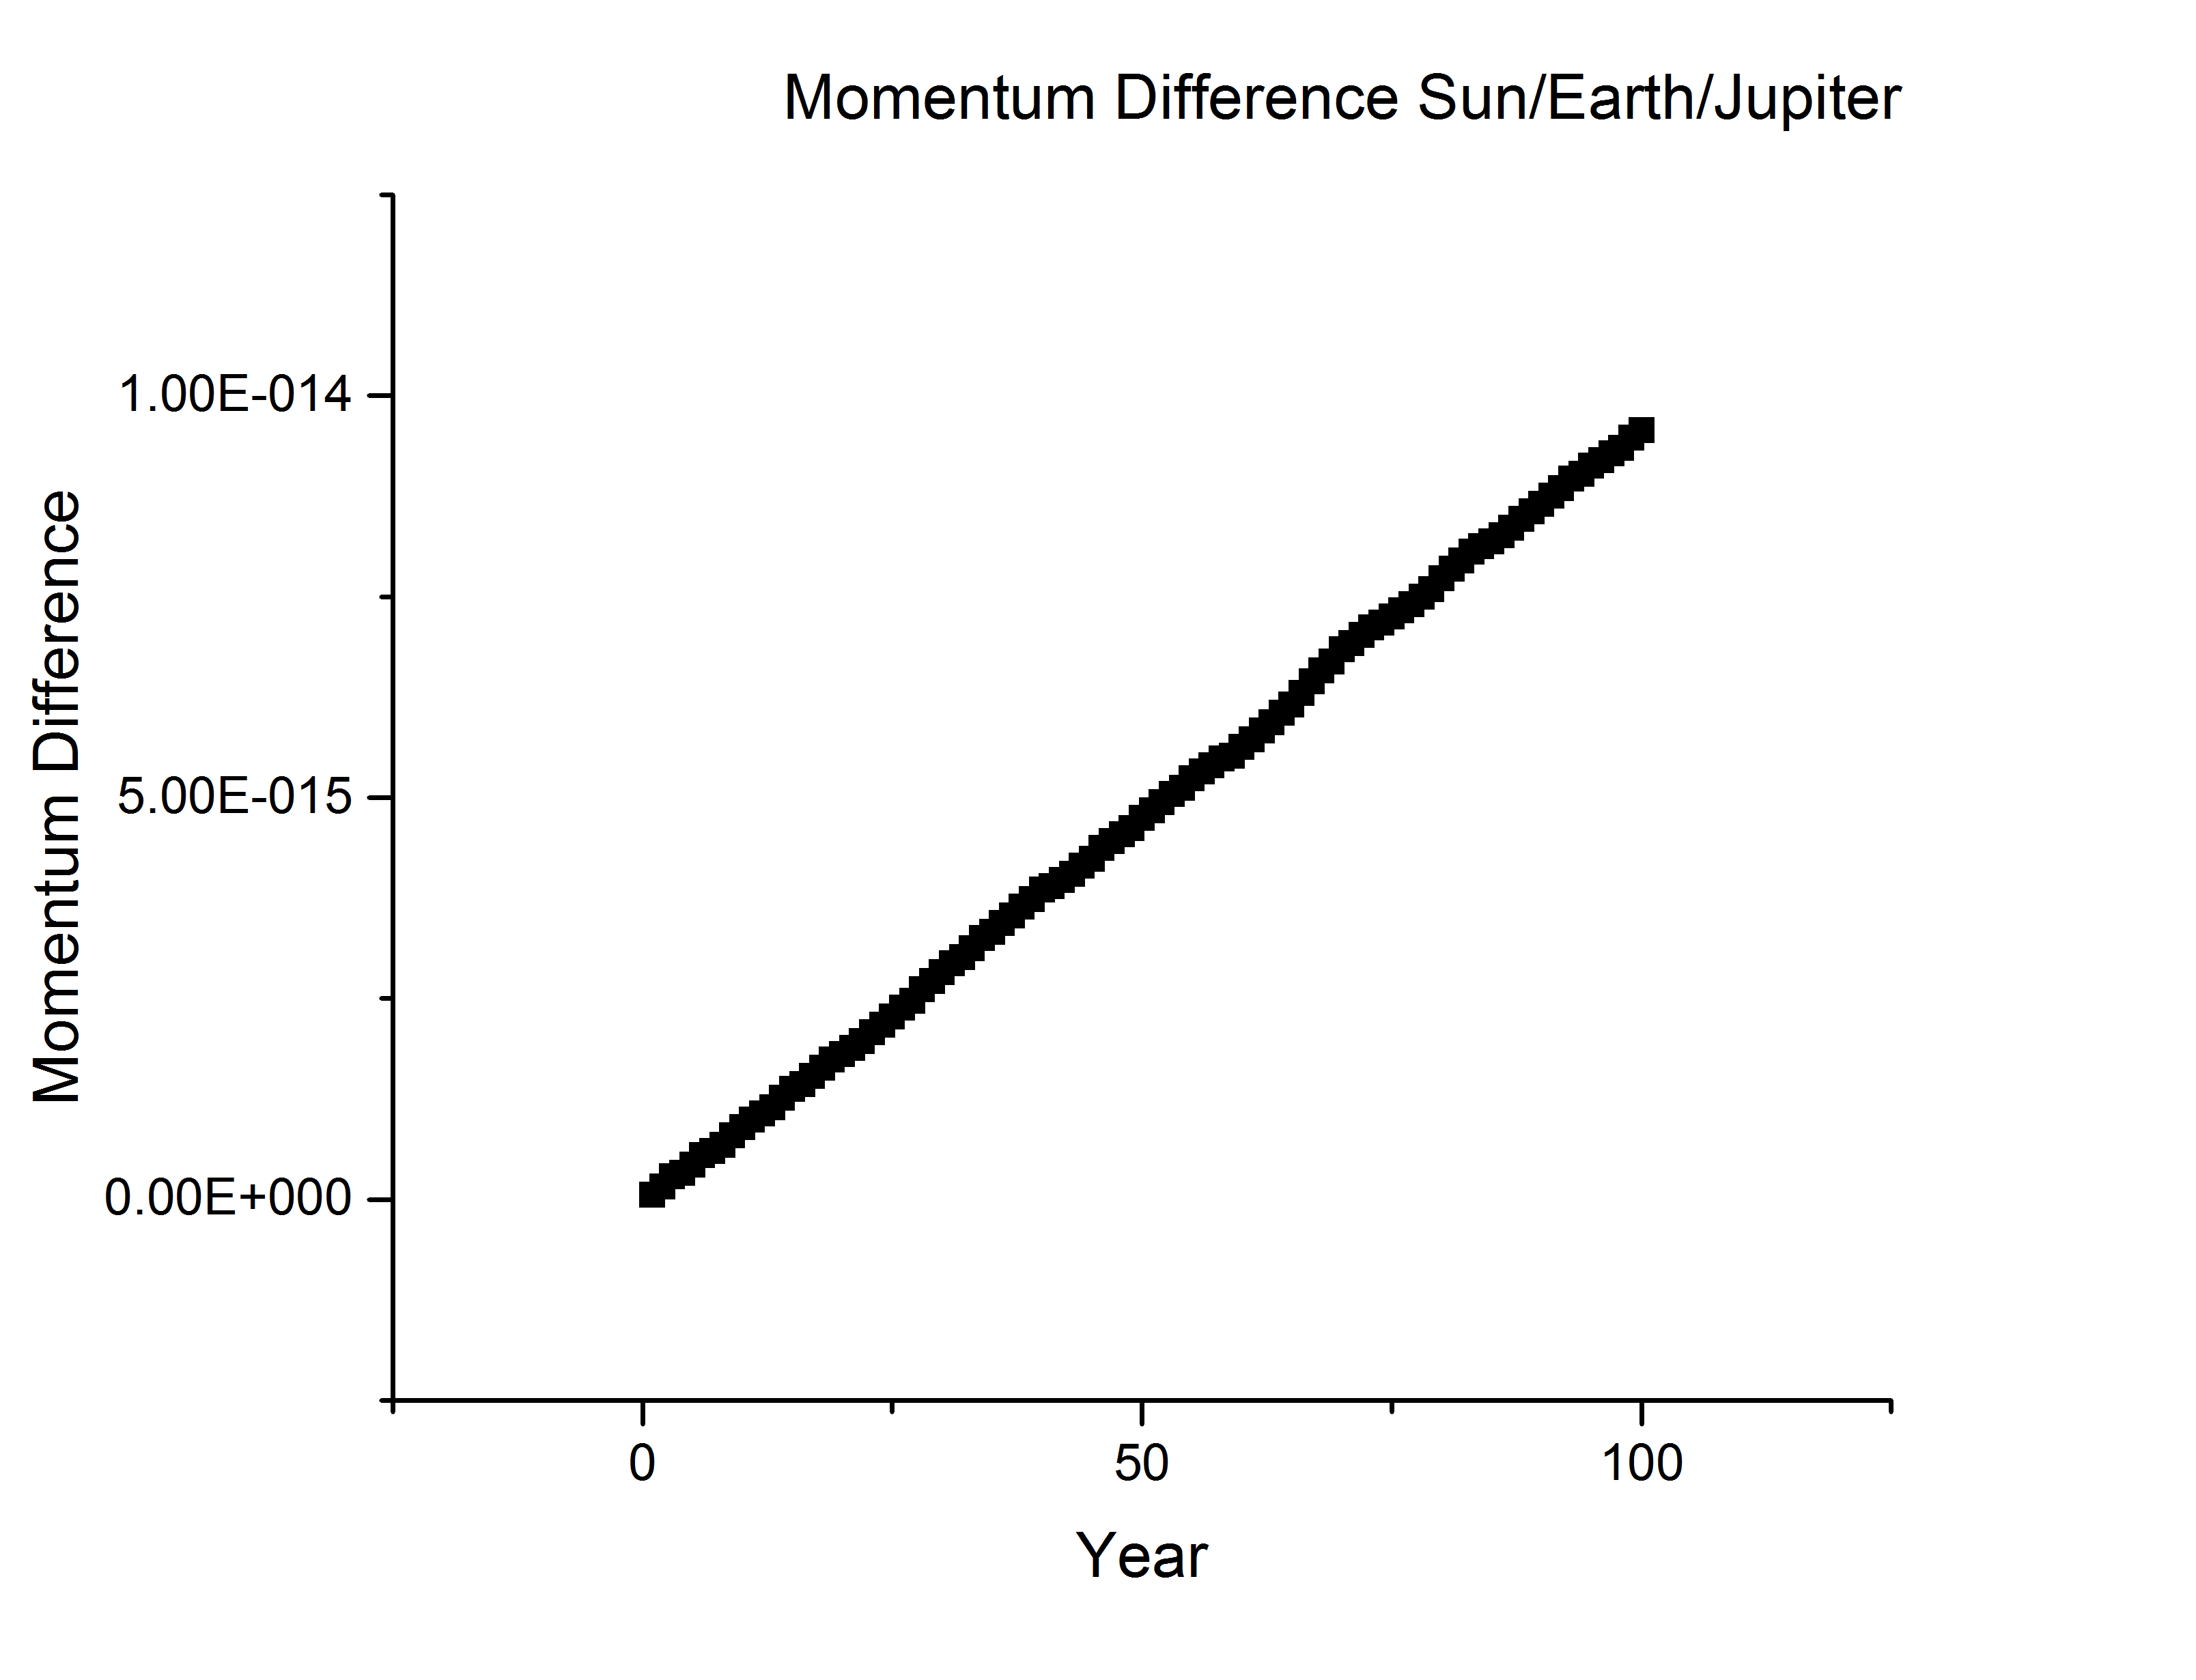
\includegraphics[scale=0.25]{Graph13.png}
	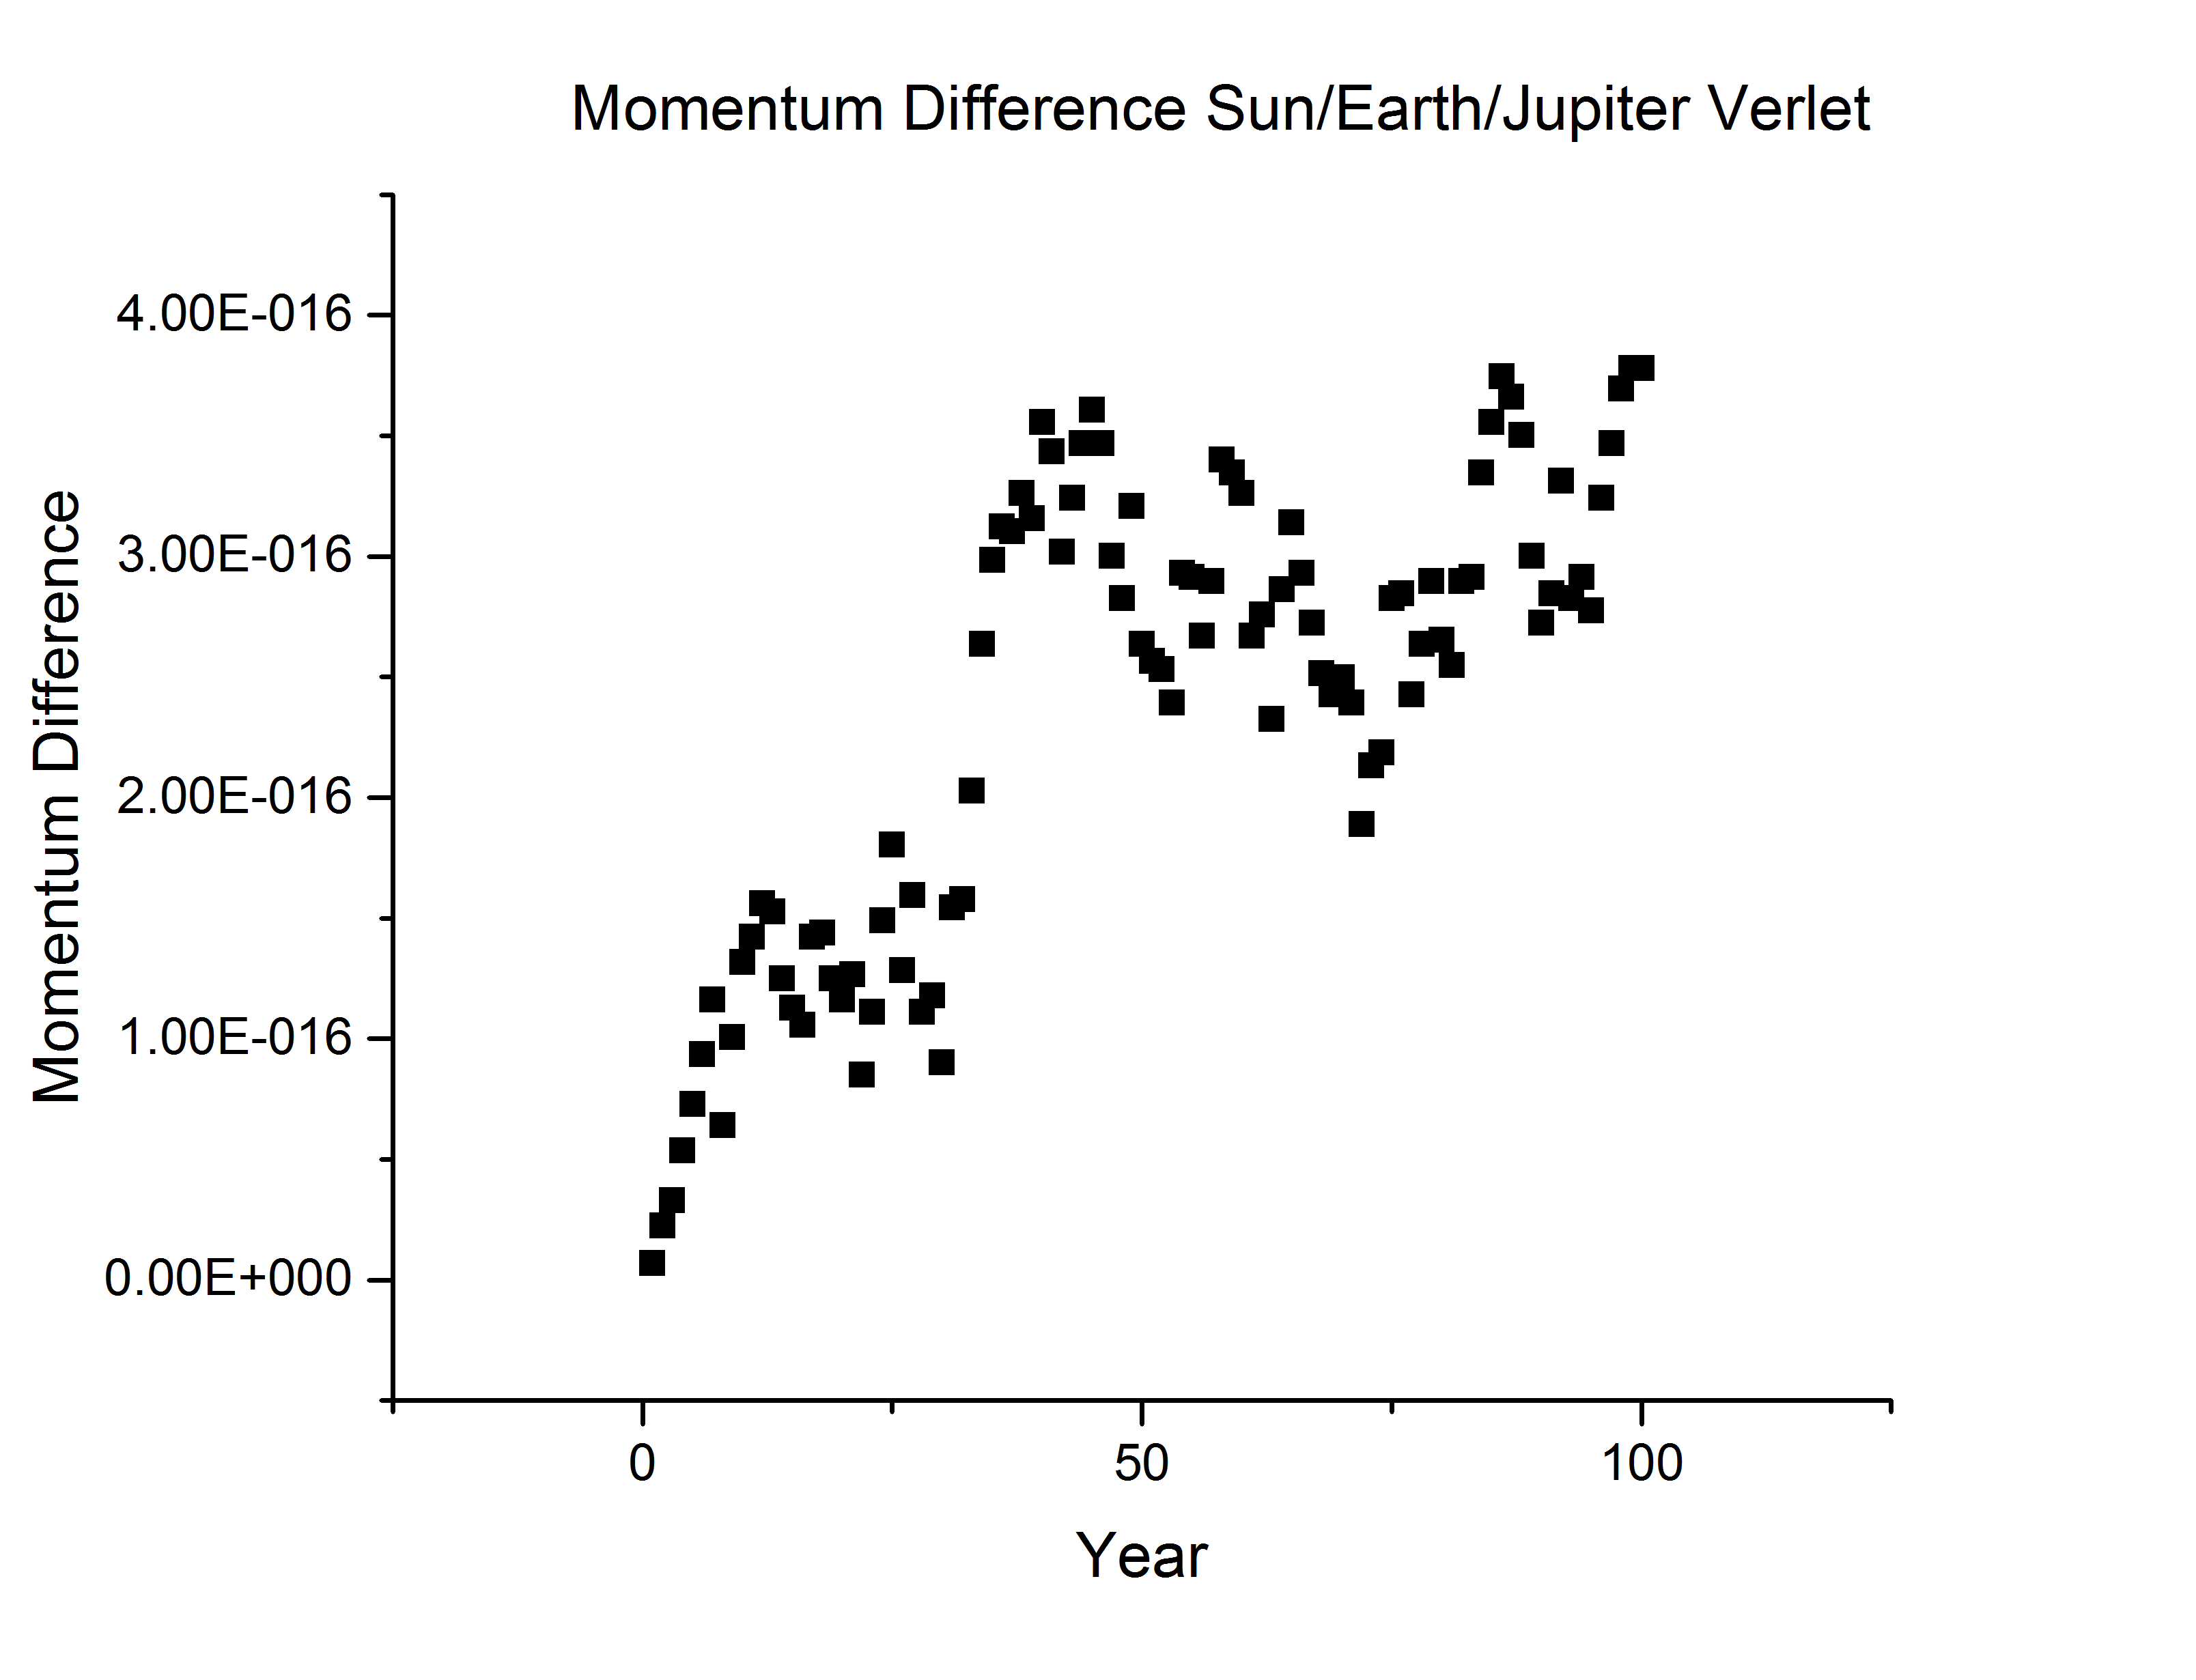
\includegraphics[scale=0.25]{Graph12.png}
		\caption{\label{Stability3} Momentum difference for Sun/Earth/Jupiter step size 0.001. }	
\end{figure}
	Changing the size of Jupiter actually didn't do very much for affecting the stability of the energy from what was discussed above, however it did disrupt the orbit of earth significantly for the case where the mass of Jupiter was 1000 times that of what it is now, actually this mass seemed to send earth flying off into outerspace after just a few orbits of the earth around the sun. Looking at it it seems that the earth actually falls into the sun before being slingshotted out into the solar system (so what this means is ouch).
	
	
			\begin{figure}
				\begin{center}
				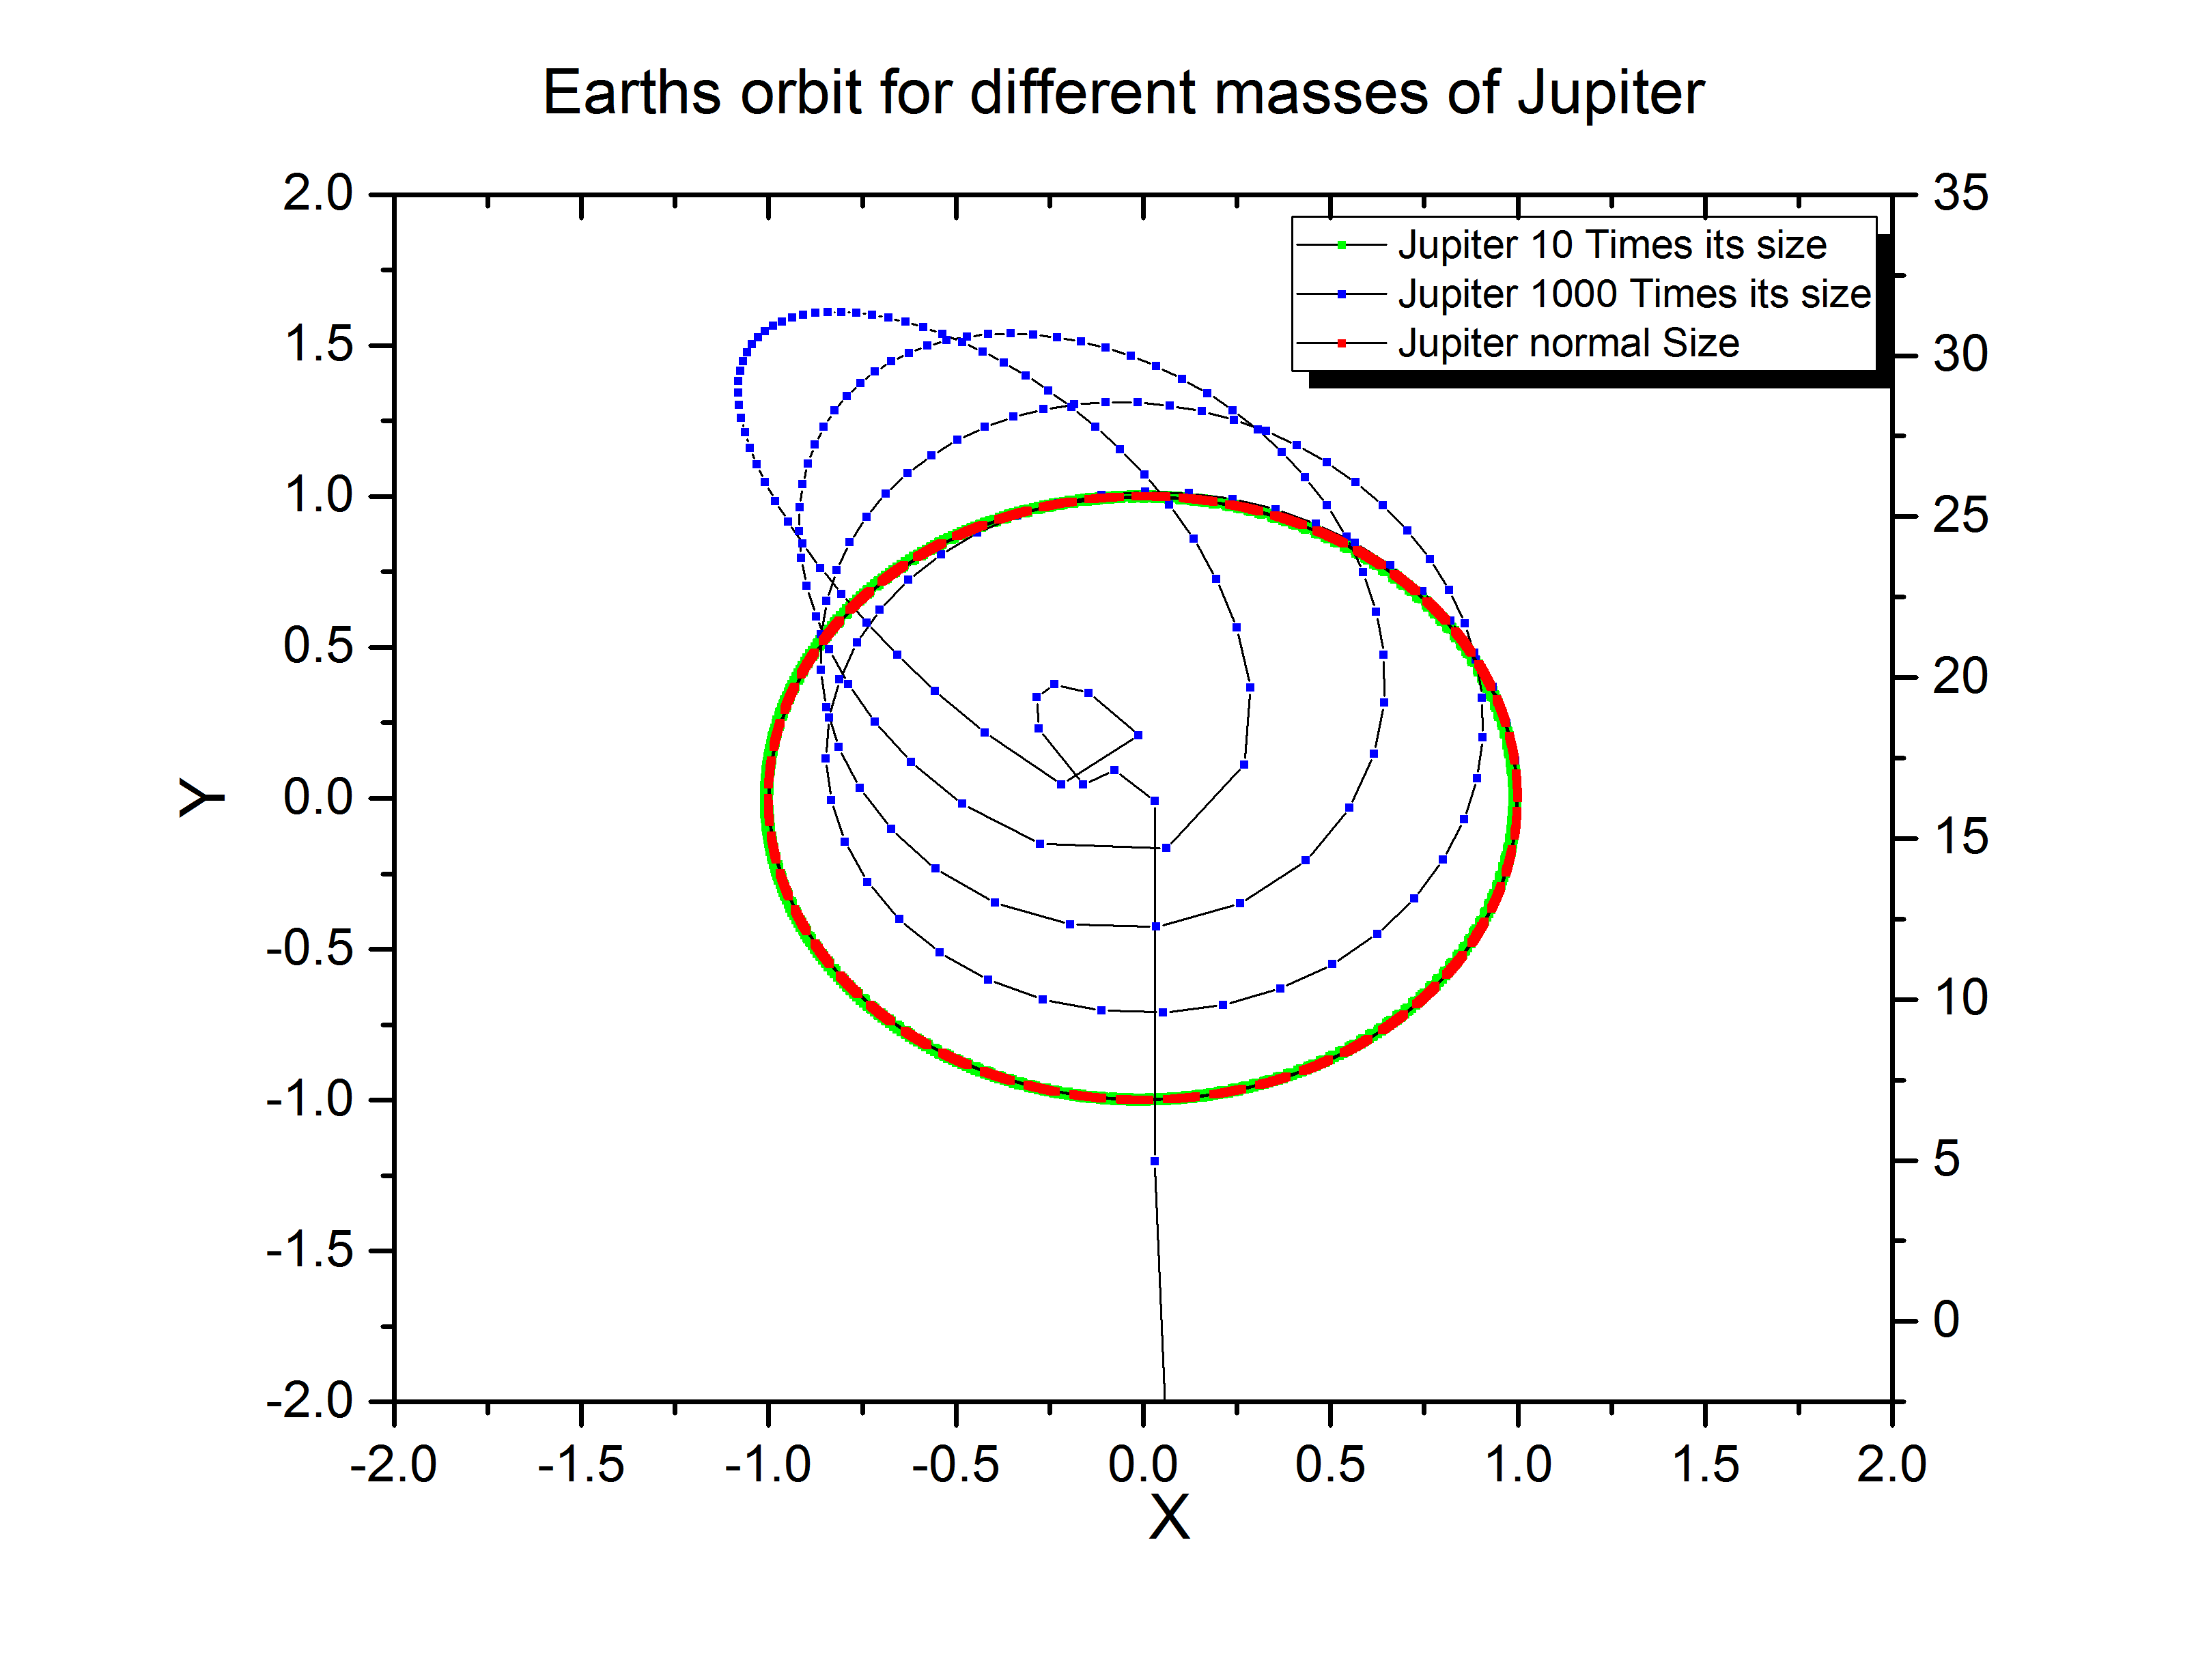
\includegraphics[scale=0.35]{Graph16.png}
					\caption{\label{SEJ} Orbits of Earth for different masses of Jupiter. }
					\end{center}
				\end{figure}
				
				The last thing to do with the system after this was to now allow the sun to move, doing so gives the following result .
				
				\begin{figure}
					\begin{center}
					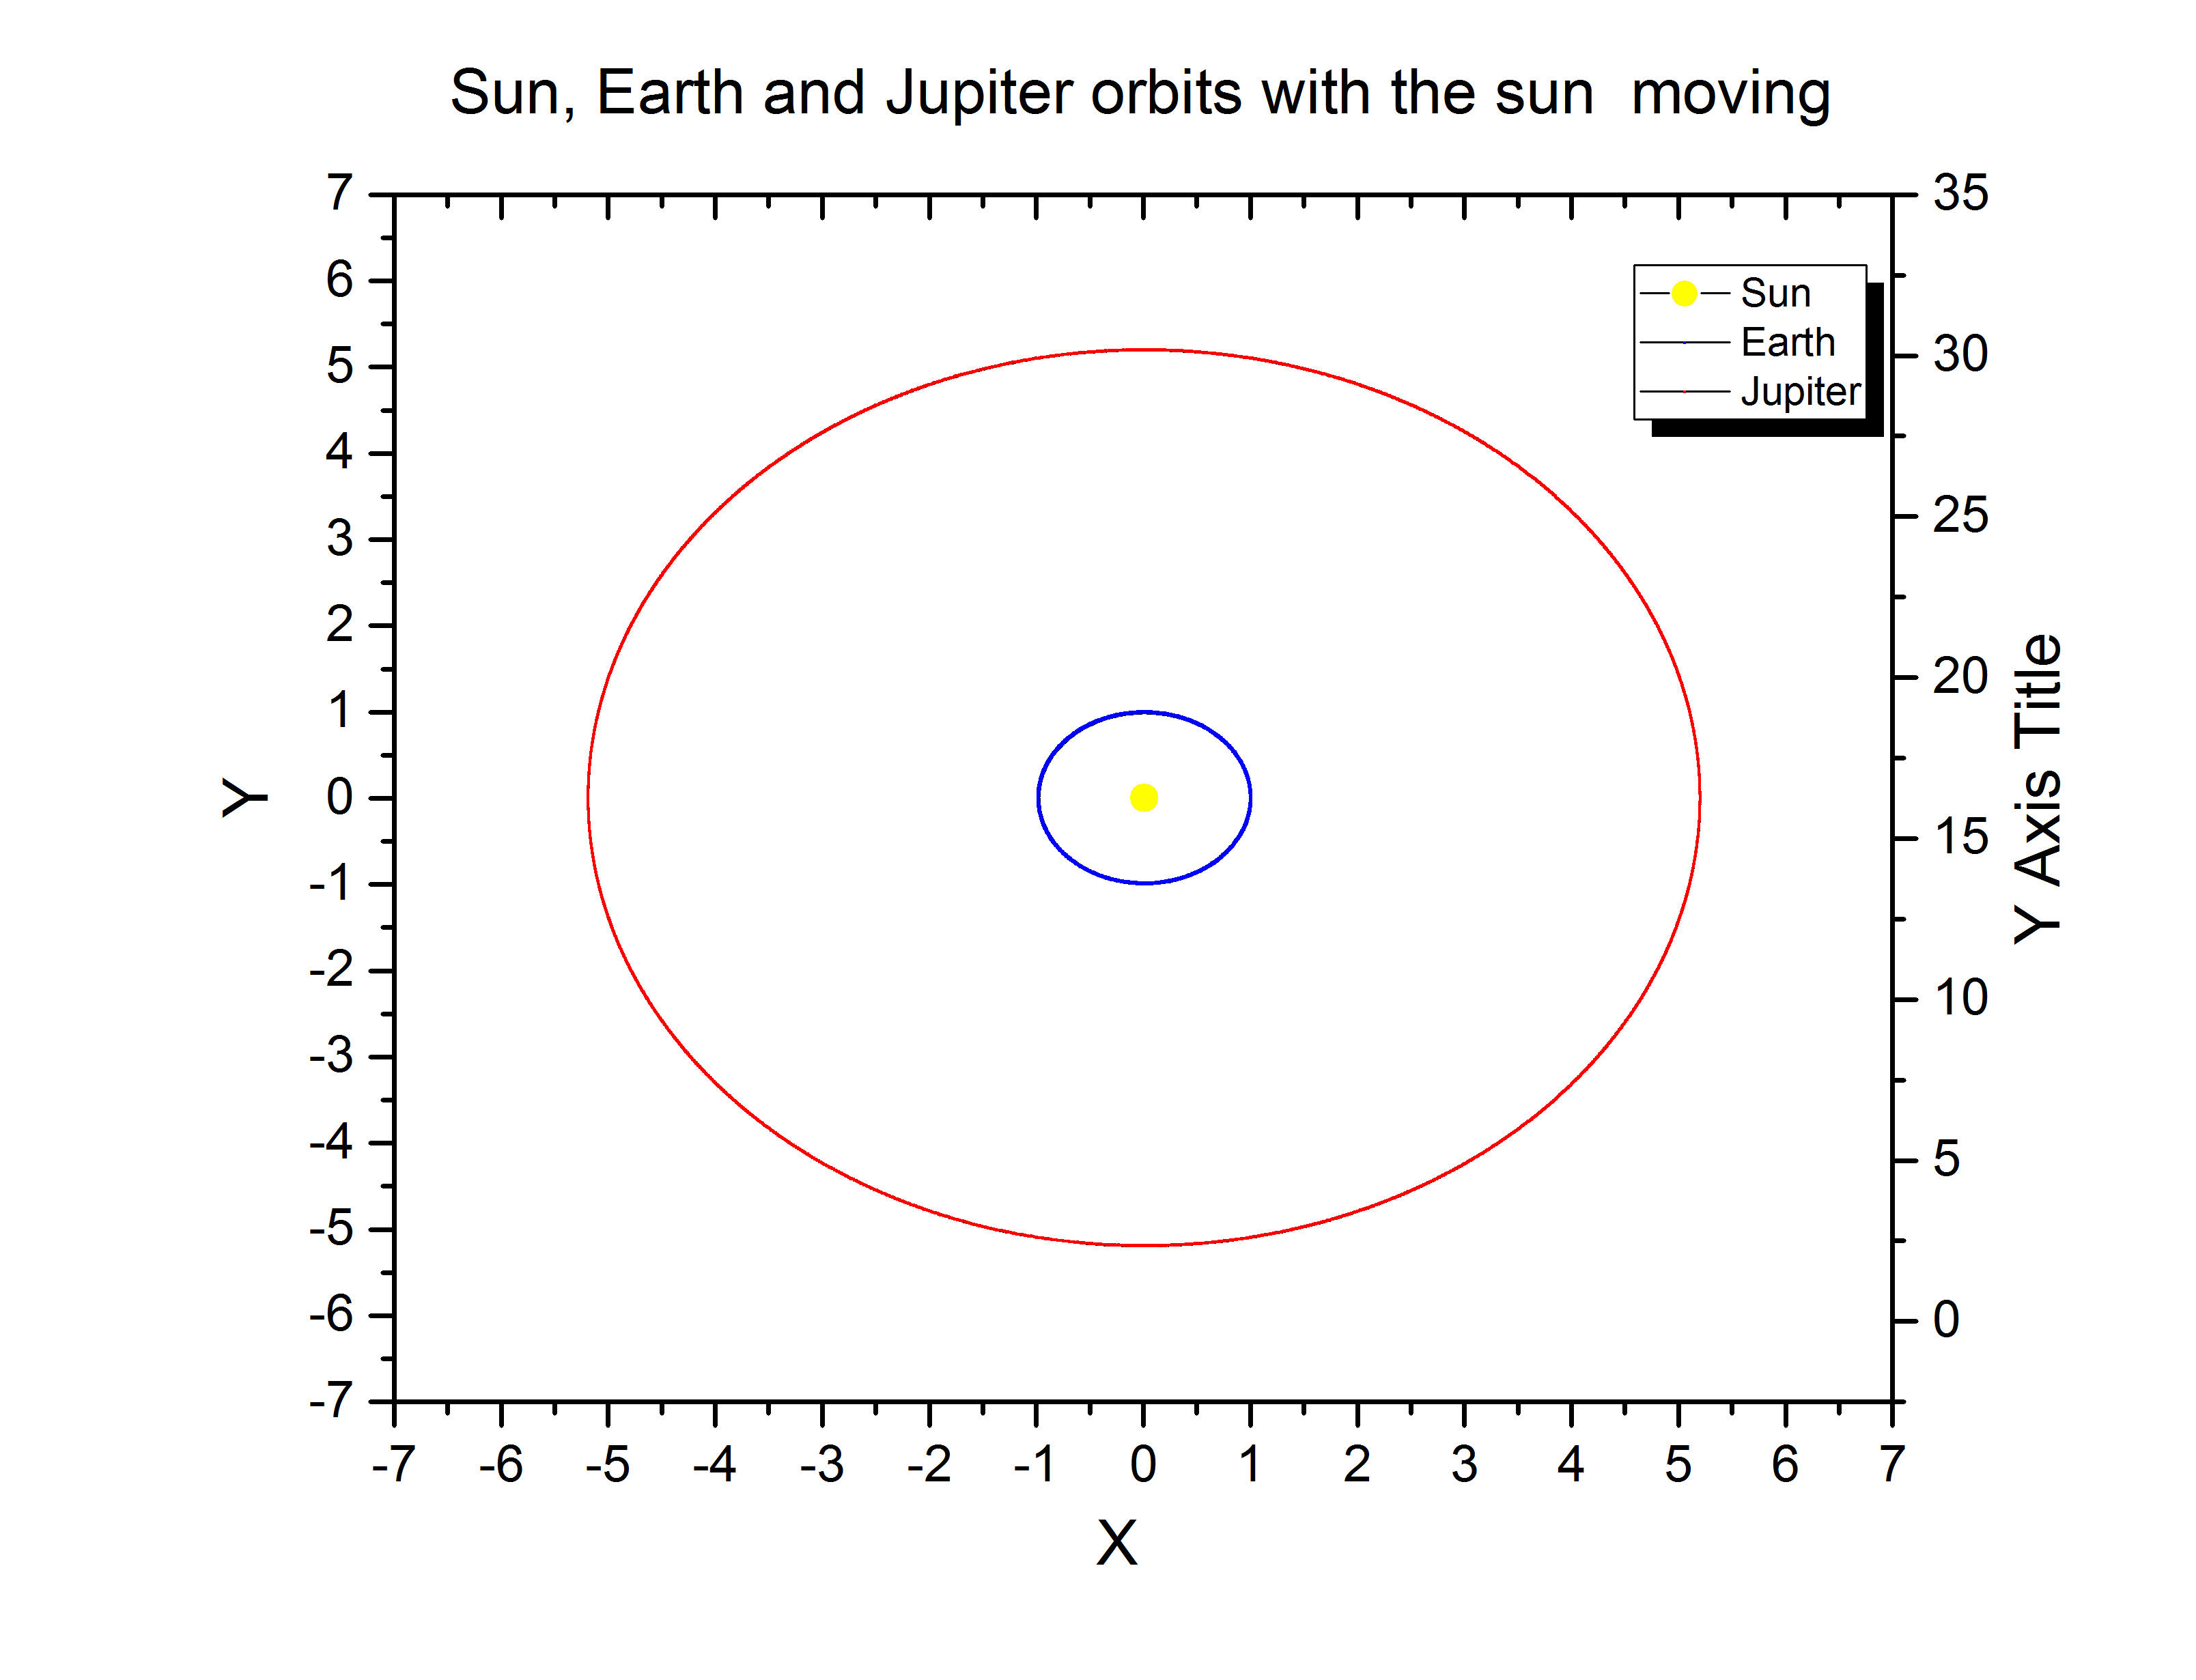
\includegraphics[scale=0.35]{Graph17.png}
					\caption{\label{SEJ2} Full 3 body system of the Sun/Earth/Jupiter. }
					\end{center}
					\end{figure}
					
\subsection{The Whole Solar System}
	The last thing to do in this project is to see how the whole solar system behaves, so adding in all of the planets and using the velocities to be from the above equation we get the following
	

	\begin{figure}
		\begin{center}
		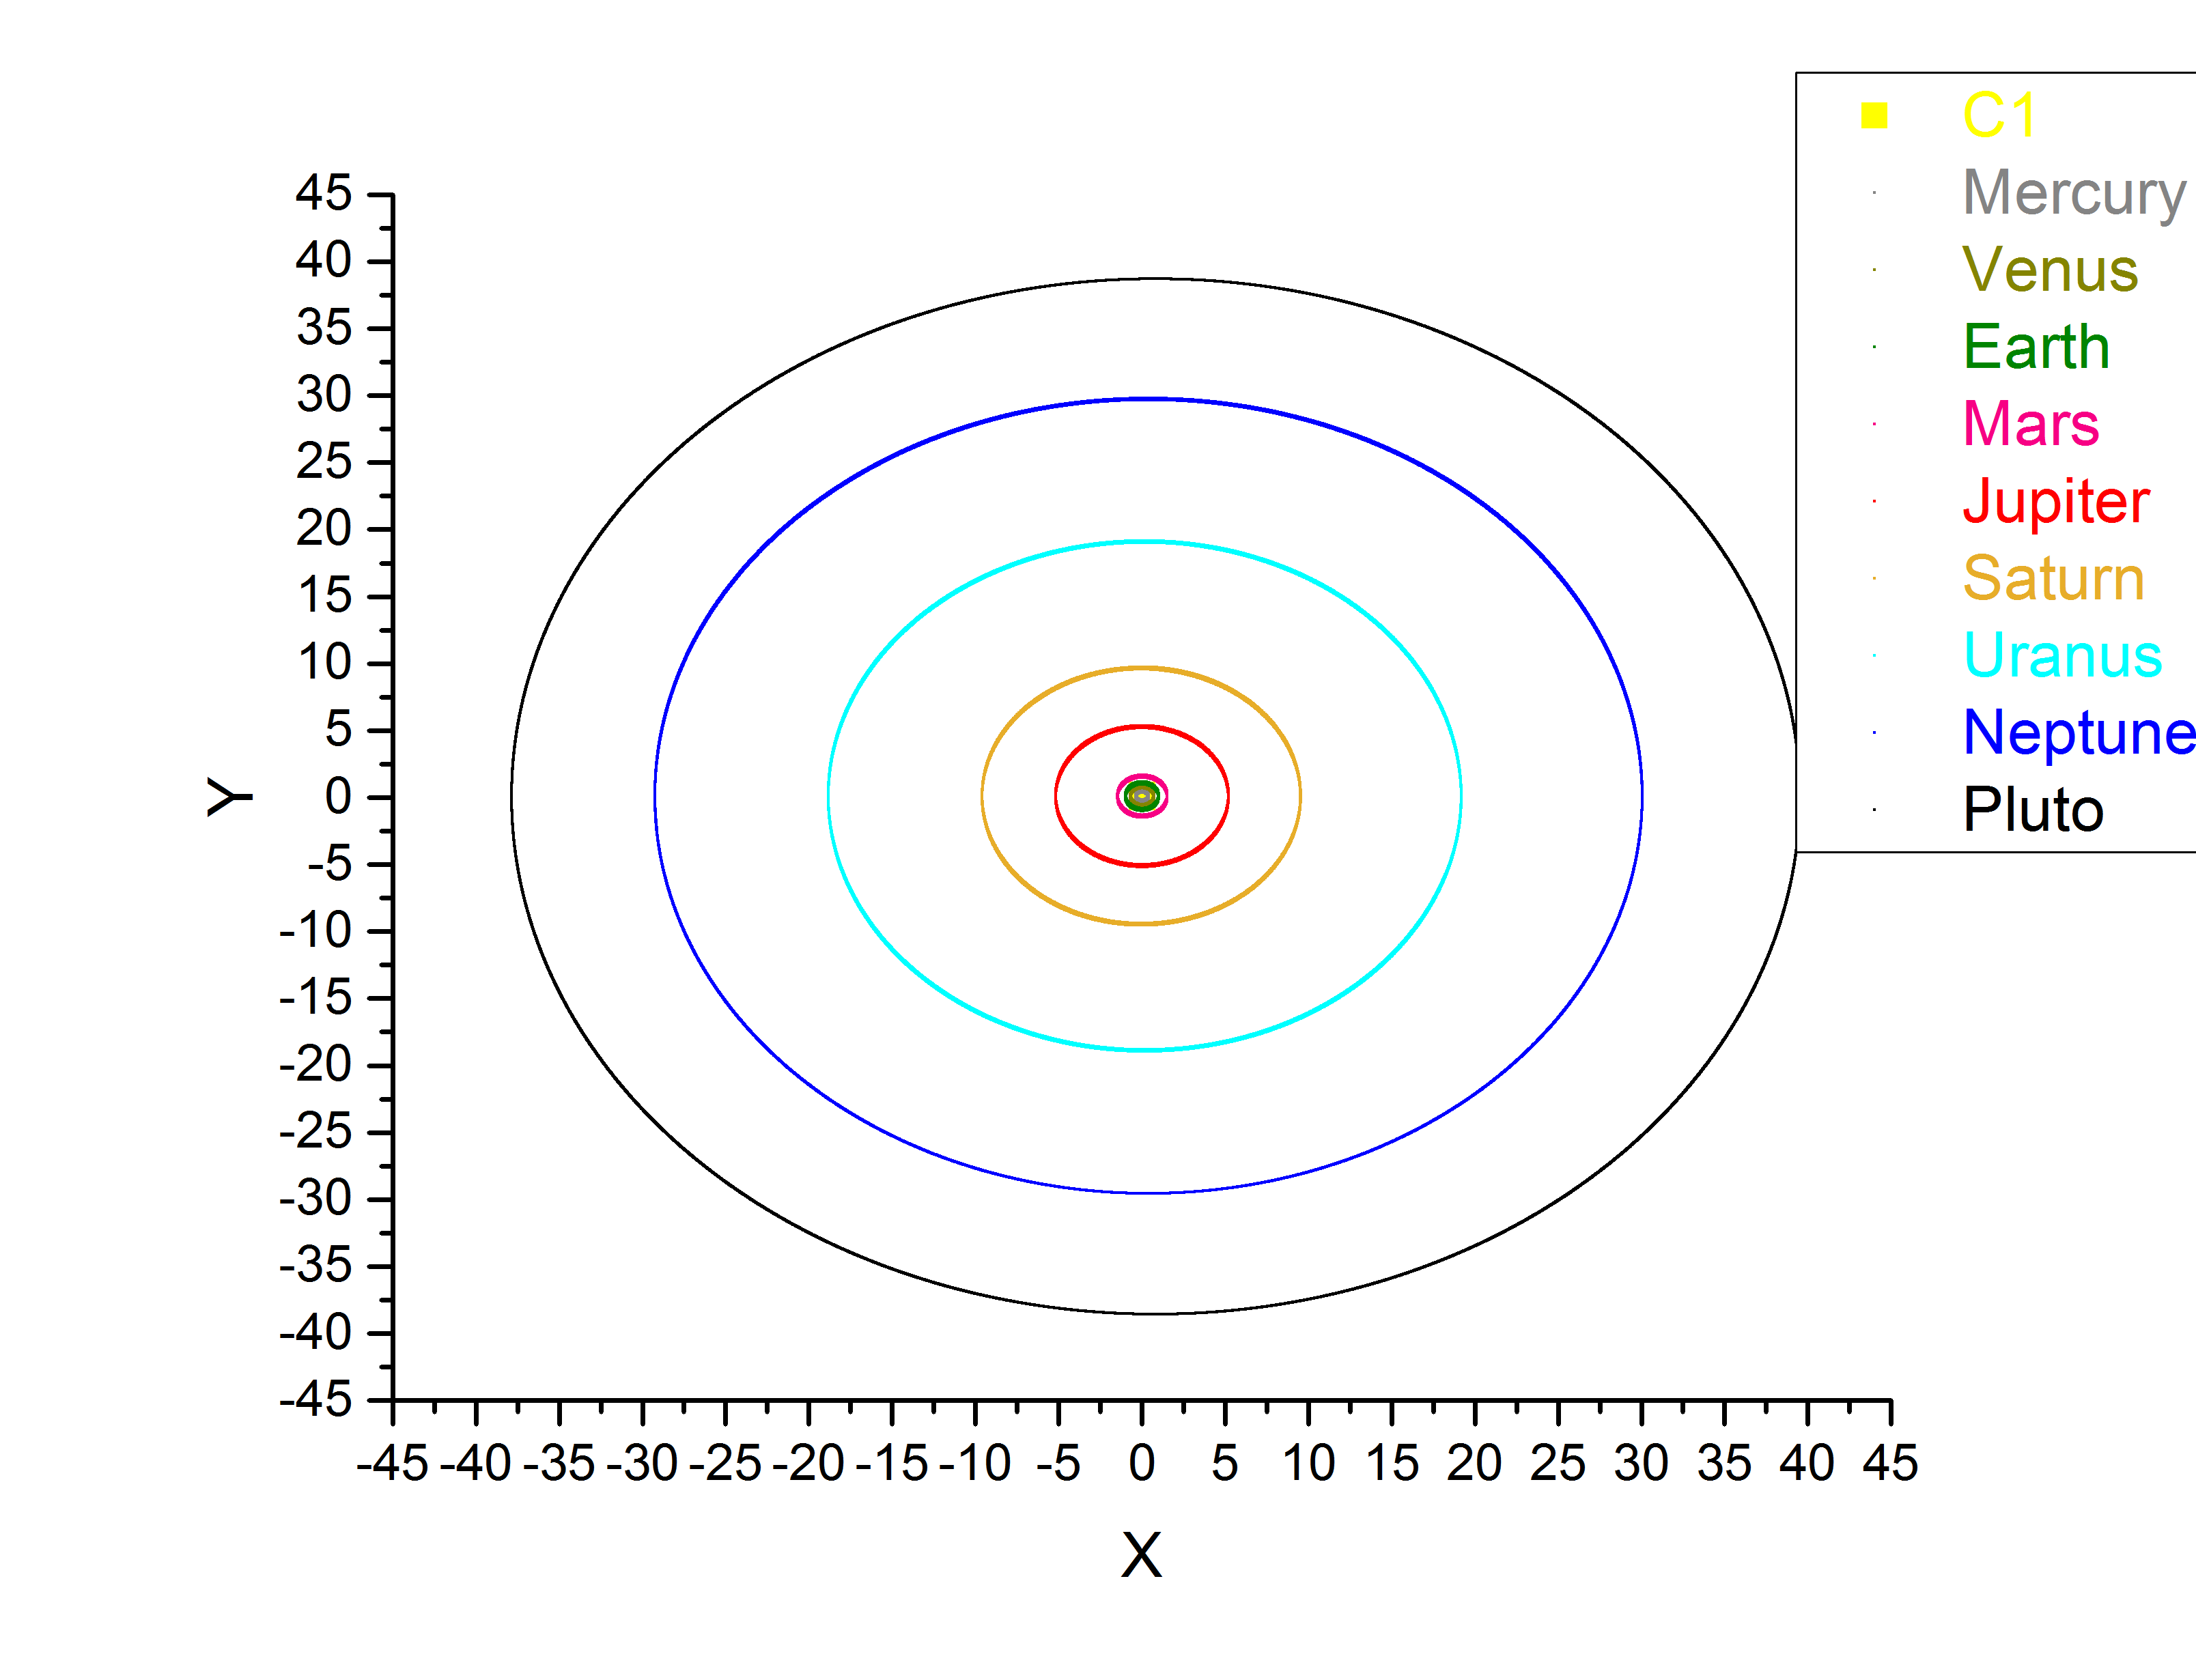
\includegraphics[scale=0.35]{Graph21.png}
			\caption{\label{SolarSystem} Orbits of the whole Solar system. }
			\end{center}
		\end{figure}
	
		Obviously Pluto's orbit is wrong since it is general knowledge that it is very elliptical and it actually crosses the orbit of Neptune, but apart from that everything seems very good. Figure 6 by the way is over the course of 500 years at a step size of 0.001, so even after that amount of time everything seems to be going fairly well. So even though our energy and momentum are not quite stable I think it is fair to say that they are stable enough to accurately depict the solar system.
		
		\subsection{Precession of Mercury}
		The final little part of this project of this project that was investigated into was to see what happened when a small change was added to the force. In Newtonian mechanics the $\frac{1}{r^2}$ force will produce orbits that line up on top of each other. However, if a small perturbation is added in this will cause the orbit to precess. For our case we looked only at Mercury and added in a small correction from general relativity which has the form of $F\frac{l^2}{r^2c^2}$. Where F is the force, l the angular momentum, r the radius and c the speed of light. To track the progress of the precession we look at how the parihelion position changes in time. To do this we simply take $tan\theta_p=\frac{y_p}{x_p}$ and solve for theta and we can see how the position of parihelion changes over time. For the measurement the code was ran for 100 Mercury years with a step size of 0.00001. Now, in running the code there was some difficulty in that in the angle of precession I kept getting an offset that I cannot explain after the first orbit which compounded linearly as the code ran. Example being that after one year the precession had gone over an angle of 0.0733 degrees, which is actually larger than what the precession should be for the entire century. However, to fix this the value of tan at this position was taken and multiplied by the number of years over which the precession had taken place. This was then subtracted from the tan value to get the actual value. Doing this I found that the precession of Mercury over the course of a century to be 0.034 degrees. This is larger than the 43 arc seconds which was stated in the project however, for the assumption that was made in how I could adjust the values I think it is fairly good. I believe the problem I was having came from using the equation for the force that was used above, which has the problem in that in it's derivation it was specifically assumed that we were dealing with circular orbits, where now we have a very elliptical orbit. 
		
		This precession that we see in the orbit can be explained by the general theory of relativity. Since Mercury is the closest planet to the sun it will be more affected by the bending of space time caused by the sun than any of the other planets. This bending will in turn change the orbit of Mercury slightly, causing its orbit to precess [5].
		
	
\section{Conclusion}



 
\begin{thebibliography}{9}
	\bibitem{1}
	H, Jensen, Project 3 Introduction
	
	\bibitem{2}
	H, Jensen, Phys 904 Lecture Notes
	
	\bibitem{3}
	Wikipedia page on Isaac Newton
	
\bibitem{4}
Thorton, Marion, Classical Dynamics of Particles and Systems. Brooks/Cole, California 2004
	
\bibitem{5}	
"Putting Relativity to the Test", archive.ncsa.illinois.edu/Cyberia/NumRel/EinsteinTest.html
	
\end{thebibliography}






\end{document}	